\section{Simulation}
\subsection{Monte Carlo Simulation}
Monte Carlo Simulation ist eine numerische Methode für statistische Simulation, die Sequenzen von Zufallszahlen benutzt, um die Simulation durchzuführen.

\textbf{Eigenschaften:}
\begin{compactitem}
	\item Monte Carlo Simulation ist ein kräftiges Instrument, um komplexe statistische Analysen durchzuführen und Wahrscheinlichkeiten und Verteilungen zu schätzen.
	\item Es verlangt ein Systemmodell (quantitative Systembeschreibung).
	\item Es werden (virtuelle) Experimente mit dem System ausgeführt, um Schlussfolgerungen bzgl. deren Verhalten zu ziehen.
\end{compactitem}

\begin{example}
	Berechne den Wert von $\pi$
	\begin{multicols}{5}
		Fläche Rechteck: $(2r)^2$ \\
		Fläche Kreis: $\pi r^2$ \\
		$\frac{\text{Fläche Rechteck}}{\text{Fläche Kreis}}$: $\frac{4}{\pi}$ \\
		$\pi$: $4 * \frac{\text{Fläche Kreis}}{\text{Fläche Rechteck}}$ \\
		$\pi$: $4 * \frac{\text{Punkte im Kreis}}{\text{Punkte im Rechteck}}$	
	\end{multicols}
	\begin{minipage}[h]{0.825\textwidth}
		\begin{lstlisting}[mathescape=true, tabsize=2]
N Punkte $X_i$ = -1 + 2$A_i$ und
N Punkte $Y_i$ = -1 + 2$B_i$ mit A, B Sequenzen von unabhaengigen Zufallszahlen
K = 0
for i = 1 : N
	if ($X_i^2$ + $Y_i^2$ < 1)
		K = K + 1
	end
end
$\pi$ = 4 * K / N
		\end{lstlisting}
	\end{minipage}
	\begin{minipage}[h]{0.175\textwidth}
		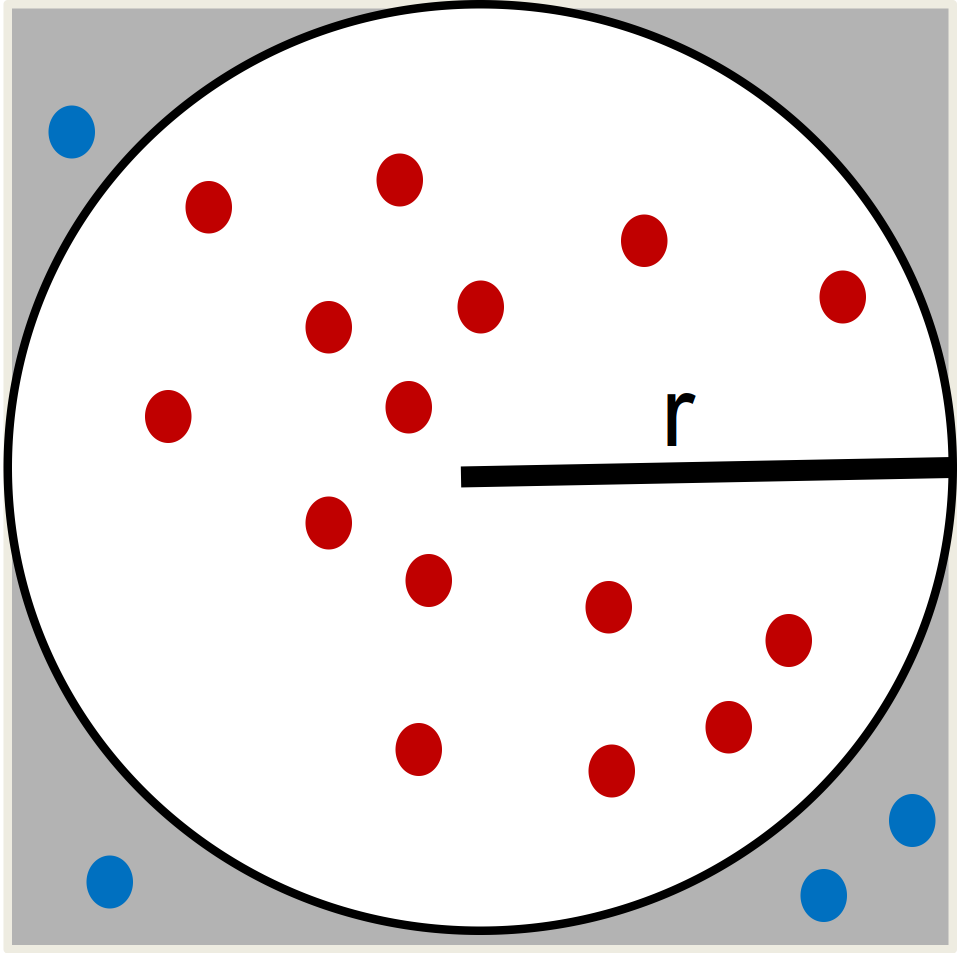
\includegraphics[width=1\textwidth]{pictures/montecarlopi}
	\end{minipage}
\end{example}

\subsection{Diskrete Ereignissimulation}
\subsubsection{Warteschlangentheorie}
Die Warteschlangentheorie beschäftigt sich mit der mathematischen Analyse von Systemen, in denen Aufträge von Bedienungsstationen bearbeitet werden und gibt Antwort auf die Fragen nach den charakteristischen Grössen, wie der Stabilität des Wartesystems, der Anzahl Kunden im System, ihrer Wartezeit etc. Sie unterstützt unter anderem Führungsentscheidungen über den Personaleinsatz und den Abfertigungsprozess. Ihre Anwendung reicht von Telekommunikationssystemen, Verkehrssystemen über Logistik bis zu Fertigungssystemen.
\begin{example}\\
	\begin{tabular}{|l|l|l|}
		\hline
		\textbf{System} & \textbf{Bedienungsstation} & \textbf{Aufträge} \\ \hline
		Bank & Schalter & Kundenbesuche \\ \hline
		Spital & Ärzte, Pflegende, Betten & Patientinnen und Patienten \\ \hline
		Rechner & CPU, I/O-Geräte & Jobs \\ \hline
		Fertigung & Maschinen, Operateure & Bauteile \\ \hline
		Rettungsdienst & Rettungsfahrzeuge, Notfallärzte & Patientinnen und Patienten \\ \hline		
	\end{tabular}
\end{example}

\subsubsection{Hauptmerkmale}
\begin{compactitem}
	\item Anwesenheit stochastischer Prozesse
	\item Zeit(-ablauf) spielt eine wichtige Rolle.
	\item Wertveränderungen der Variablen werden verursacht durch Ereignisse und treten nur an diskreten Zeitpunkten auf.
\end{compactitem}

\begin{multicols}{2}
	\textbf{Vorteile:}
	\begin{compactitem}
		\item Kostengünstiges und sicheres Experimentierfeld
		\item Ermöglicht Analyse komplexer Systeme durch hohen Detaillierungsgrad
		\item Ermöglicht Animation und steigert somit Systemverständnis
	\end{compactitem}
	\textbf{Nachteile:}
	\begin{compactitem}
		\item Erfordert einen hohen initialen Zeitaufwand
		\item Bau eines Simulationsmodells ist relativ fehleranfällig
		\item Interpretation der Analysedaten ist anspruchsvoll
	\end{compactitem} \ \\
\end{multicols}

\subsubsection{M/M/1 Modell}
\begin{multicols}{3}
	\begin{compactitem}[$\bullet$]
		\item M-Elemente betreten Warteschlange
		\item M-Elemente sind in Warteschlange
		\item 1-Element verlässt Warteschlange
	\end{compactitem}
\end{multicols}
\begin{example}\\
	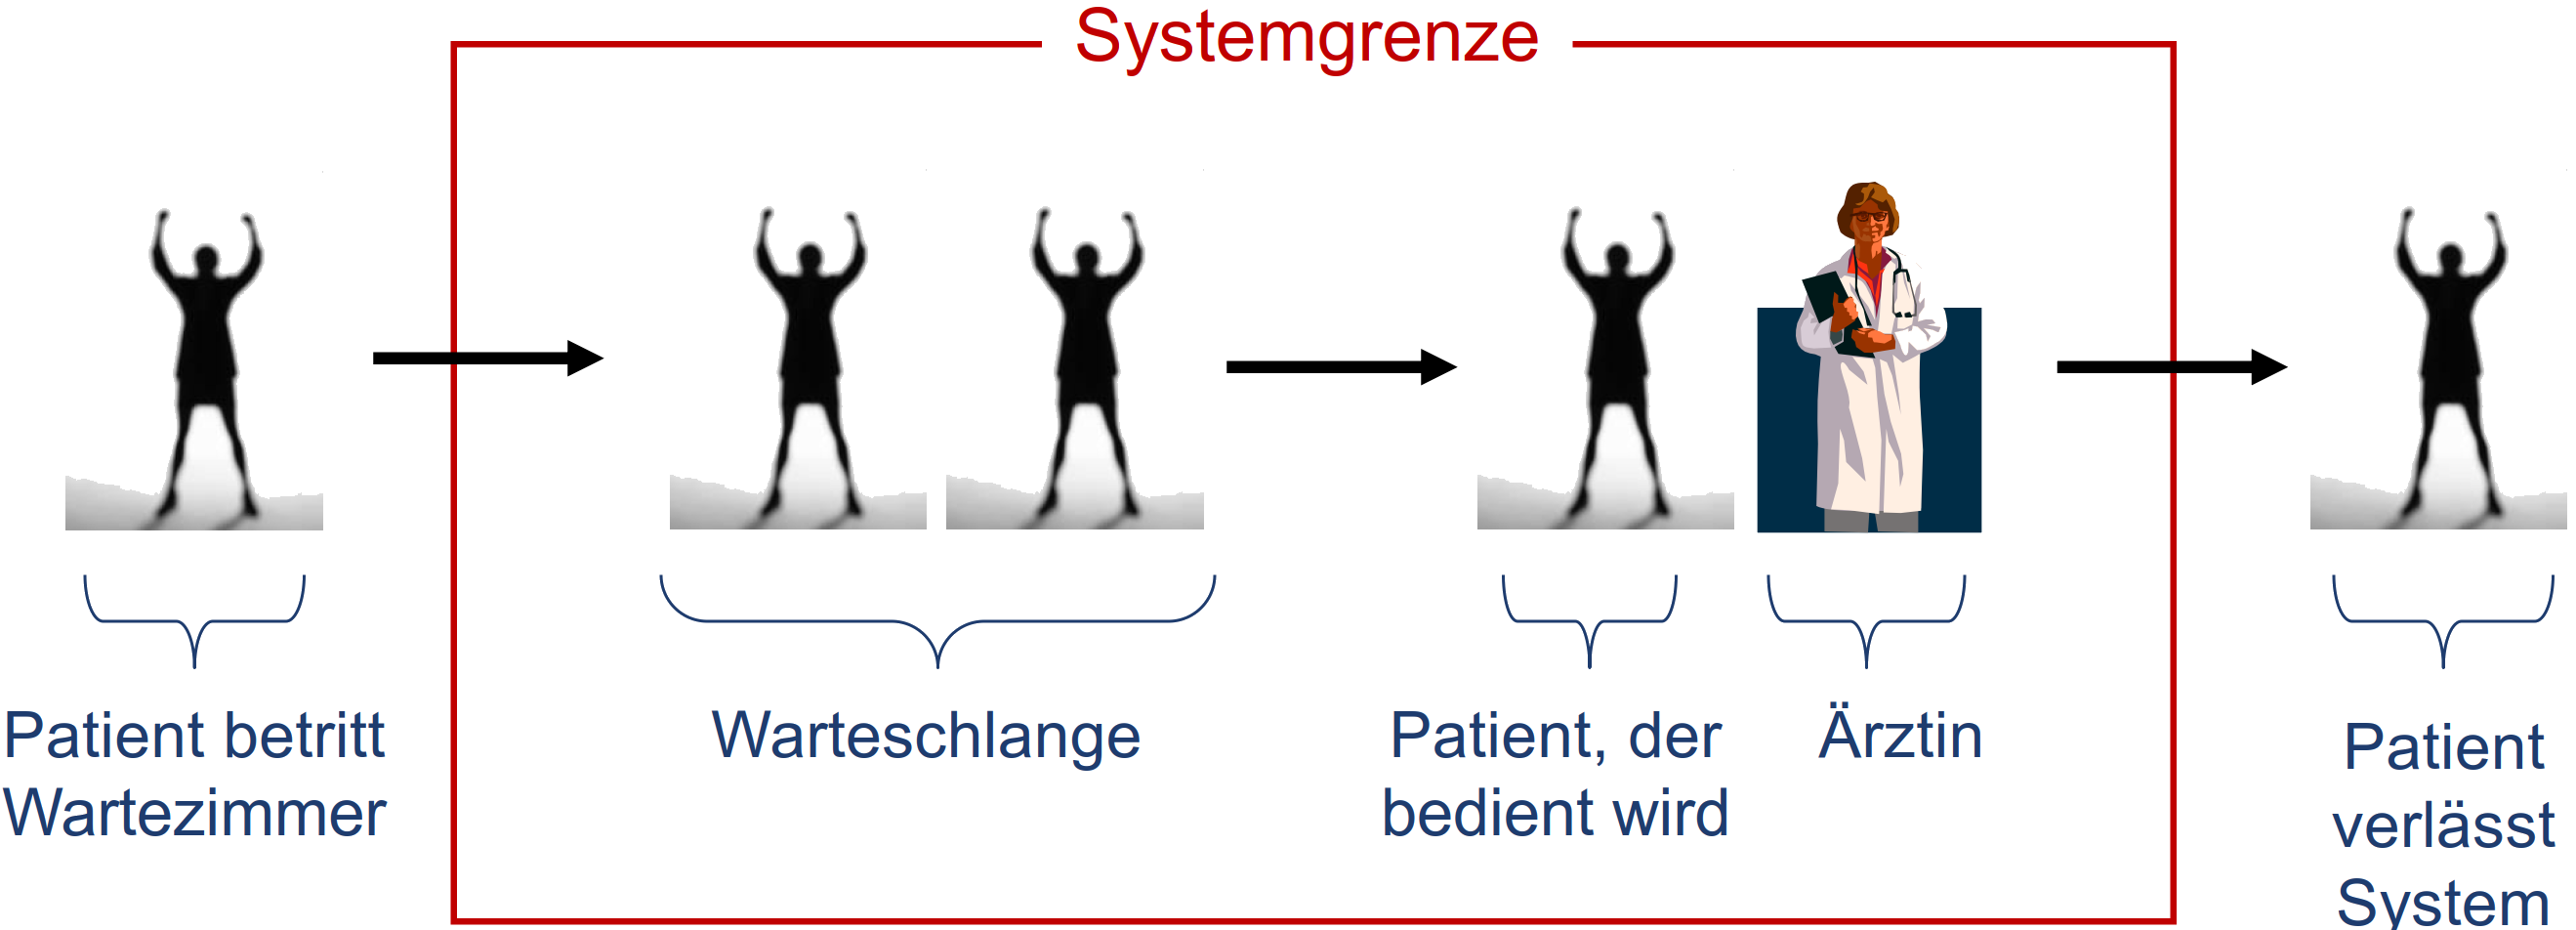
\includegraphics[width=0.7\textwidth]{pictures/mm1modell}
\end{example}
\todo{Folie 32 - Diagramme allenfalls noch einfügen}

\subsubsection{Kernelemente}
\textbf{Items:} Objekte, die durch das System fliessen (z.B. Patienten, Erstzteile, ...). Items haben meistens Attribute (Ankunftszeit, Bearbeitungsstartzeit, Prioritätsklasse, usw.). \\
\textbf{Systemzustand:} Der Zustand $Z(t)$ gibt eine vollständige Beschreibung des Systems am Zeitpunkt $t$. Der Systemzustand ist meistens ein (mehrdimensionaler) Vektor und dient u.a. der Berechnung der Zielgrössen. \\
\textbf{Simulationsuhr:} Die Simulationsuhr hält die virtuelle Zeit im Simulationsmodell fest. \\
\textbf{Ereignis:} Jedes Ereignis hat eine Wirkung, die zum Auftretenszeitpunkt ausgeübt wird. Die Wirkung besteht aus einer Änderung des Systemzustands und/oder einer Änderung der Future-Event-List. In der Zeit zwischen zwei nachfolgenden Ereignissen passiert im System nichts (der Systemzustand ändert sich nicht). Aus diesem Grund kann die Simulationsuhr von Ereignis zu Ereignis springen. \\
\textbf{Future Event List:} Dynamische Liste, die 0 oder mehr (Zeitpunkt-, Ereignis-) Paare enthält; Sie umfasst alle Ereignisse, die zum aktuellen Zeitpunkt bekannt sind. Während eines Simulationslaufs werden ständig neue Ereignisse hinzugefügt und verarbeitete Ereignisse gelöscht.

\subsubsection{Spezifikation eines DE Modells}
DE Modelle werden spezifiziert durch
\begin{compactenum}
	\item Flussdiagramme
	\item Ereignisdiagramme
\end{compactenum}

\begin{example}[Beispiel für nachfolgende Kapitel 4.2.6 - 4.2.7]
	Wir betrachten eine Maschine, worauf genau ein Produkt hergestellt wird. Der Ankunftsprozess der Produktionsaufträge ist poissonverteilt mit dem Parameterwert $\lambda$. Bearbeitungszeiten sind exponentialverteilt mit dem Parameterwert $\mu$.\\
	Bei der Produktion können Fehler auftreten. Beim Maschinenausgang werden die Produkte visuell kontrolliert. Die Wahrscheinlichkeit eines Fehlers ist $\epsilon$. Misslungene Produktionsaufträge müssen wiederholt werden. \\
	\textbf{Items:} Produktionsaufträge mit Attributen: Ankunftszeit, Bearbeitungsstartzeit, Bearbeitungszeit, Anzahl Fehlversuche, etc. \\
	\textbf{Zustand:} $Z$ = (Anzahl) Produktionsaufträge im System \\
	\textbf{Ereignisse:} $e_1$ = Ankunft eines Produktionsauftrags; $e_2$ = Bearbeitung auf der Maschine abgeschlossen
\end{example}

\subsubsection{Flussdiagramm}
\textbf{Grundbausteine:}
\begin{multicols}{5}
	Quelle und Senke: \\ \\
	Fluss: \\ \\
	Weiche: \\ \\
	Warteschlange: \\ \\
	Aktivität oder Ressource:
\end{multicols}	
\begin{multicols}{5}
	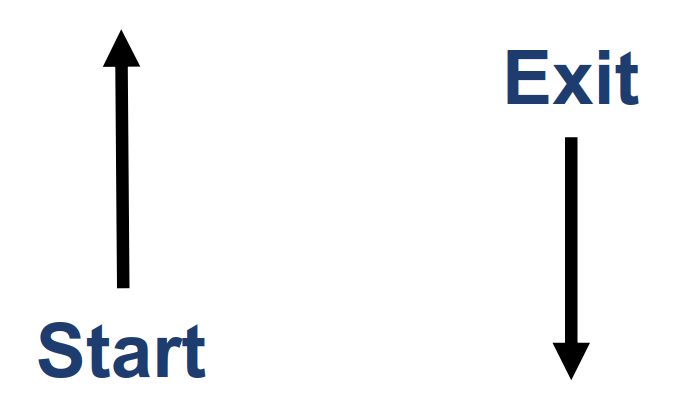
\includegraphics[width=0.15\textwidth]{pictures/fluss_quelle_senke}\\ \\
	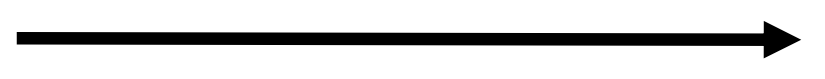
\includegraphics[width=0.15\textwidth]{pictures/fluss_fluss}\\
	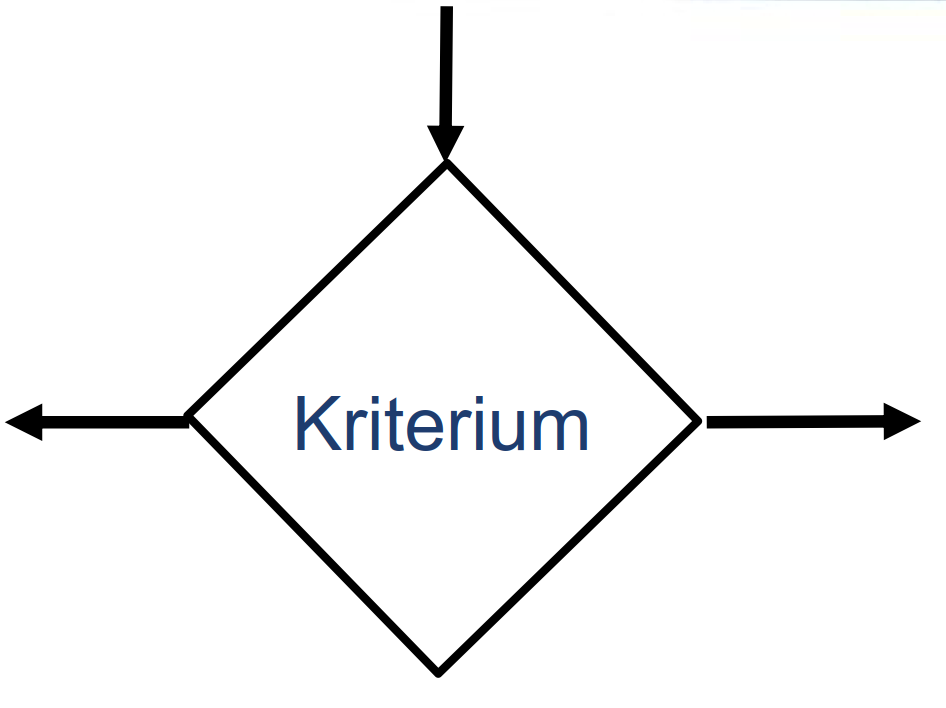
\includegraphics[width=0.15\textwidth]{pictures/fluss_weiche}\\ 
	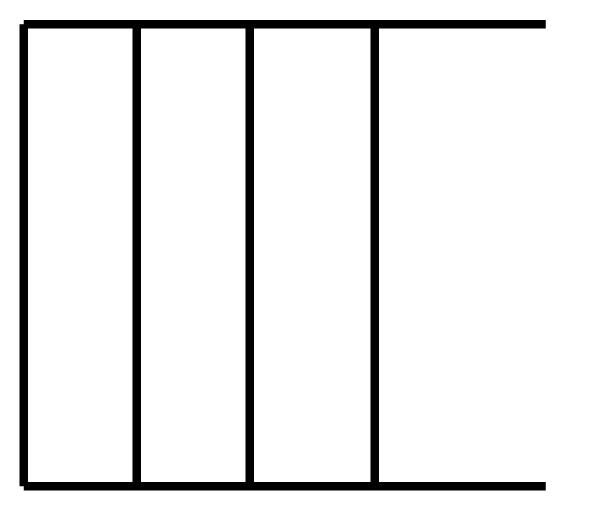
\includegraphics[width=0.1\textwidth]{pictures/fluss_warteschlange}\\ 
	
\includegraphics[width=0.15\textwidth]{pictures/fluss_aktivitaet}
\end{multicols}
\begin{multicols}{2}
	\begin{multicols}{2}
		Gabelung (konvergent):\\
		Gabelung (divergent):
	\end{multicols}
	Lager:
\end{multicols}
\begin{multicols}{2}
	\begin{multicols}{2}
		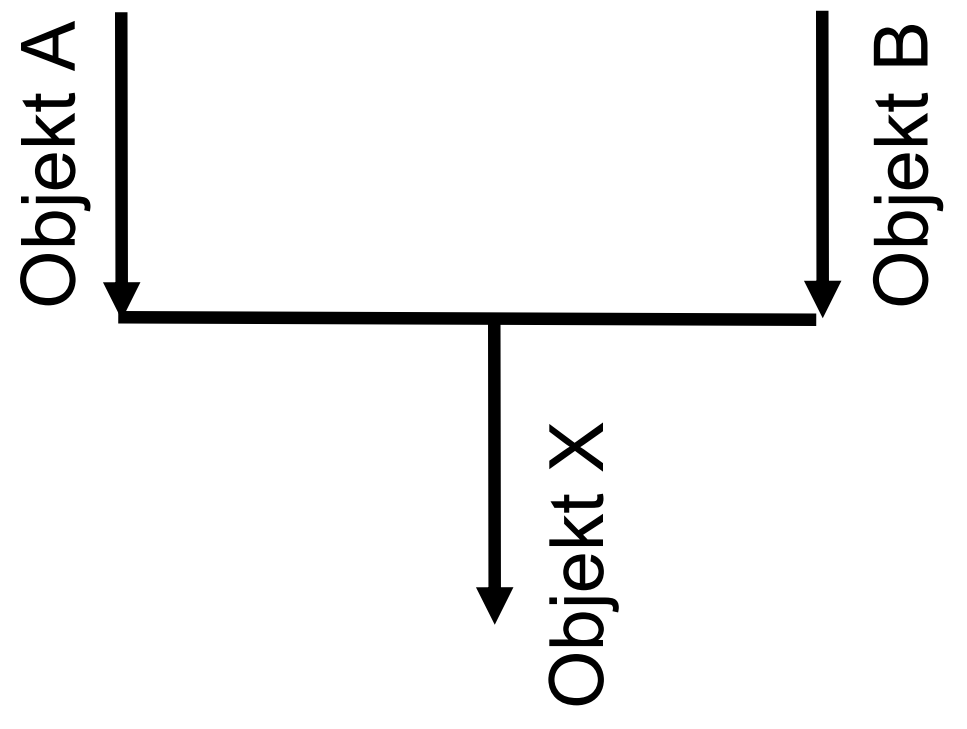
\includegraphics[width=0.2\textwidth]{pictures/fluss_gabelung1}\\ 
		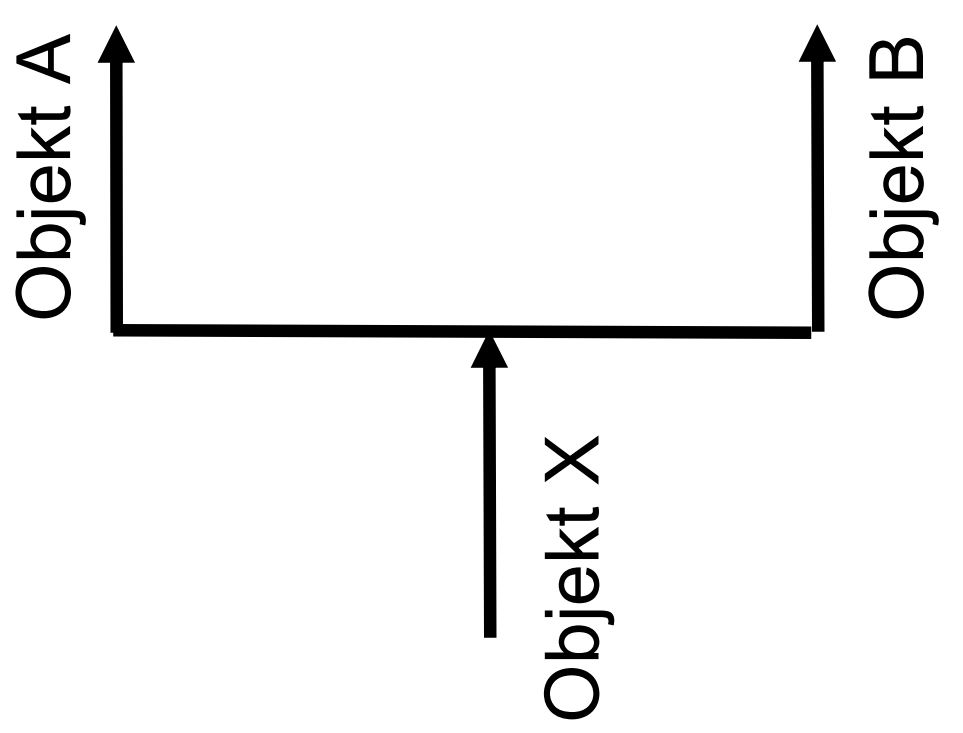
\includegraphics[width=0.2\textwidth]{pictures/fluss_gabelung2}
	\end{multicols}
	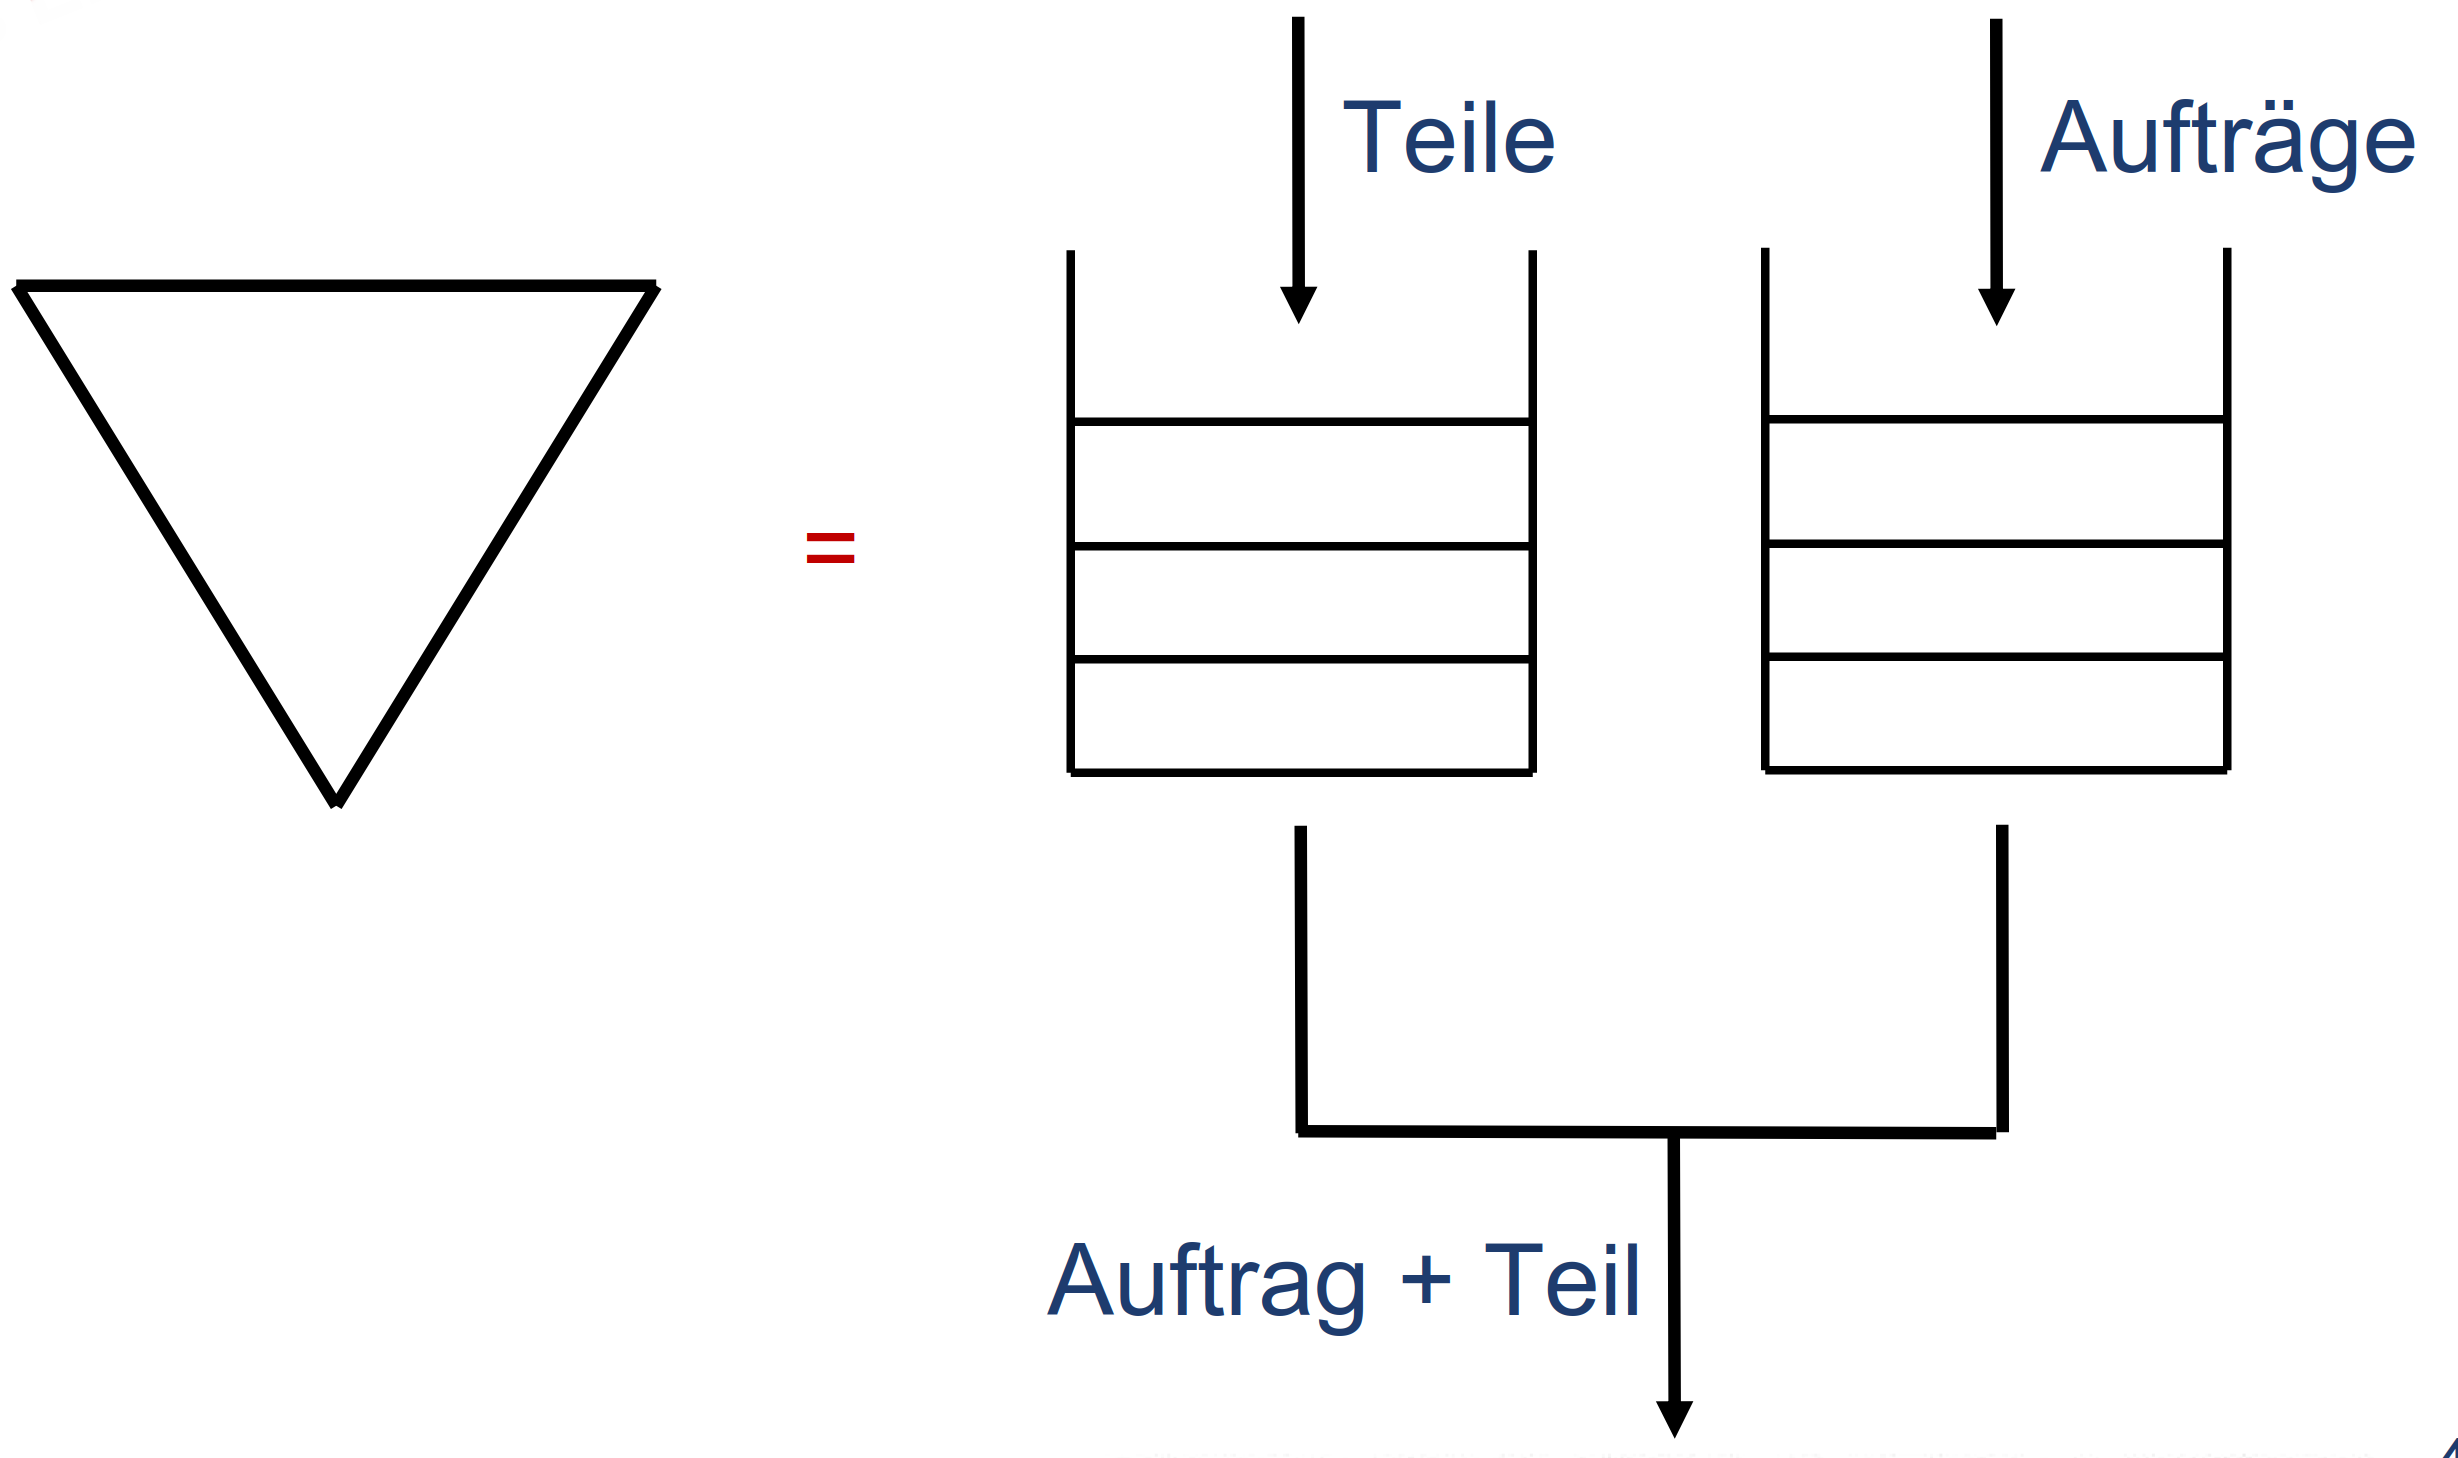
\includegraphics[width=0.4\textwidth]{pictures/fluss_lager}
\end{multicols}
\begin{example} \\
	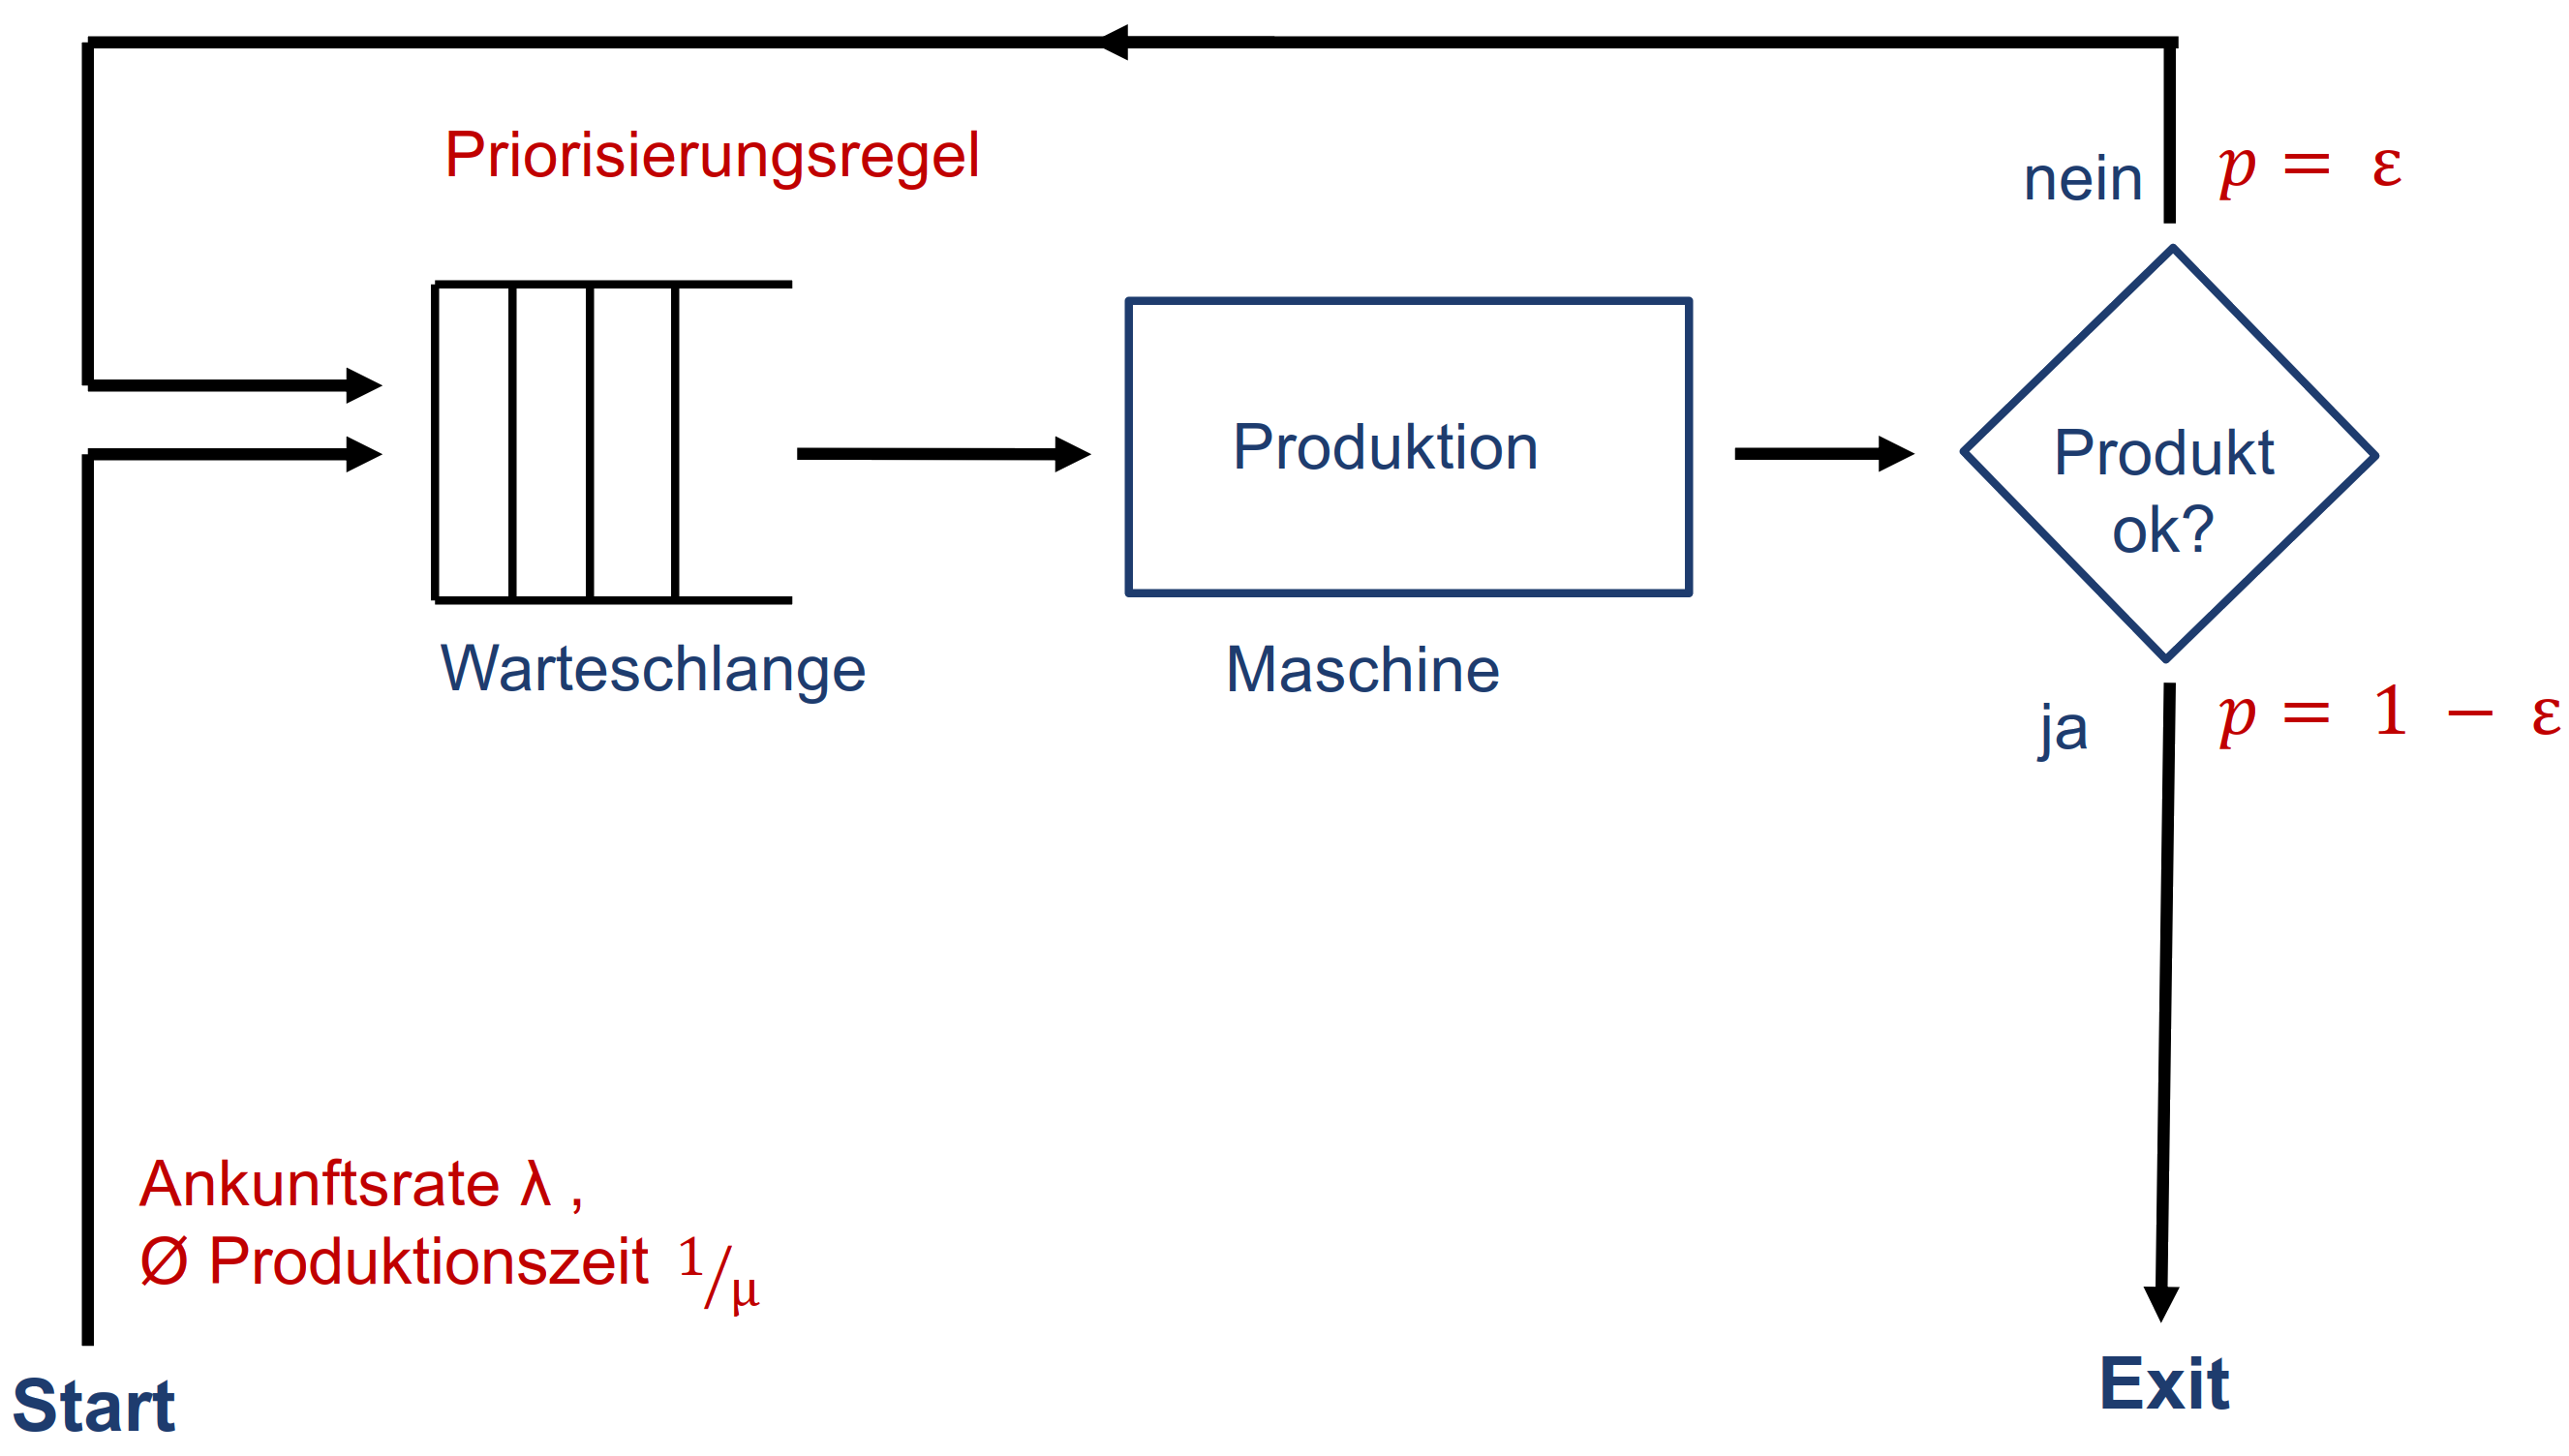
\includegraphics[width=0.5\textwidth]{pictures/flussdiagramm}
\end{example}

\subsubsection{Ereignisdiagramm}
\begin{example} 
	\begin{multicols}{2}
		\textbf{Ereignisdiagramm $e_1$:} \\
		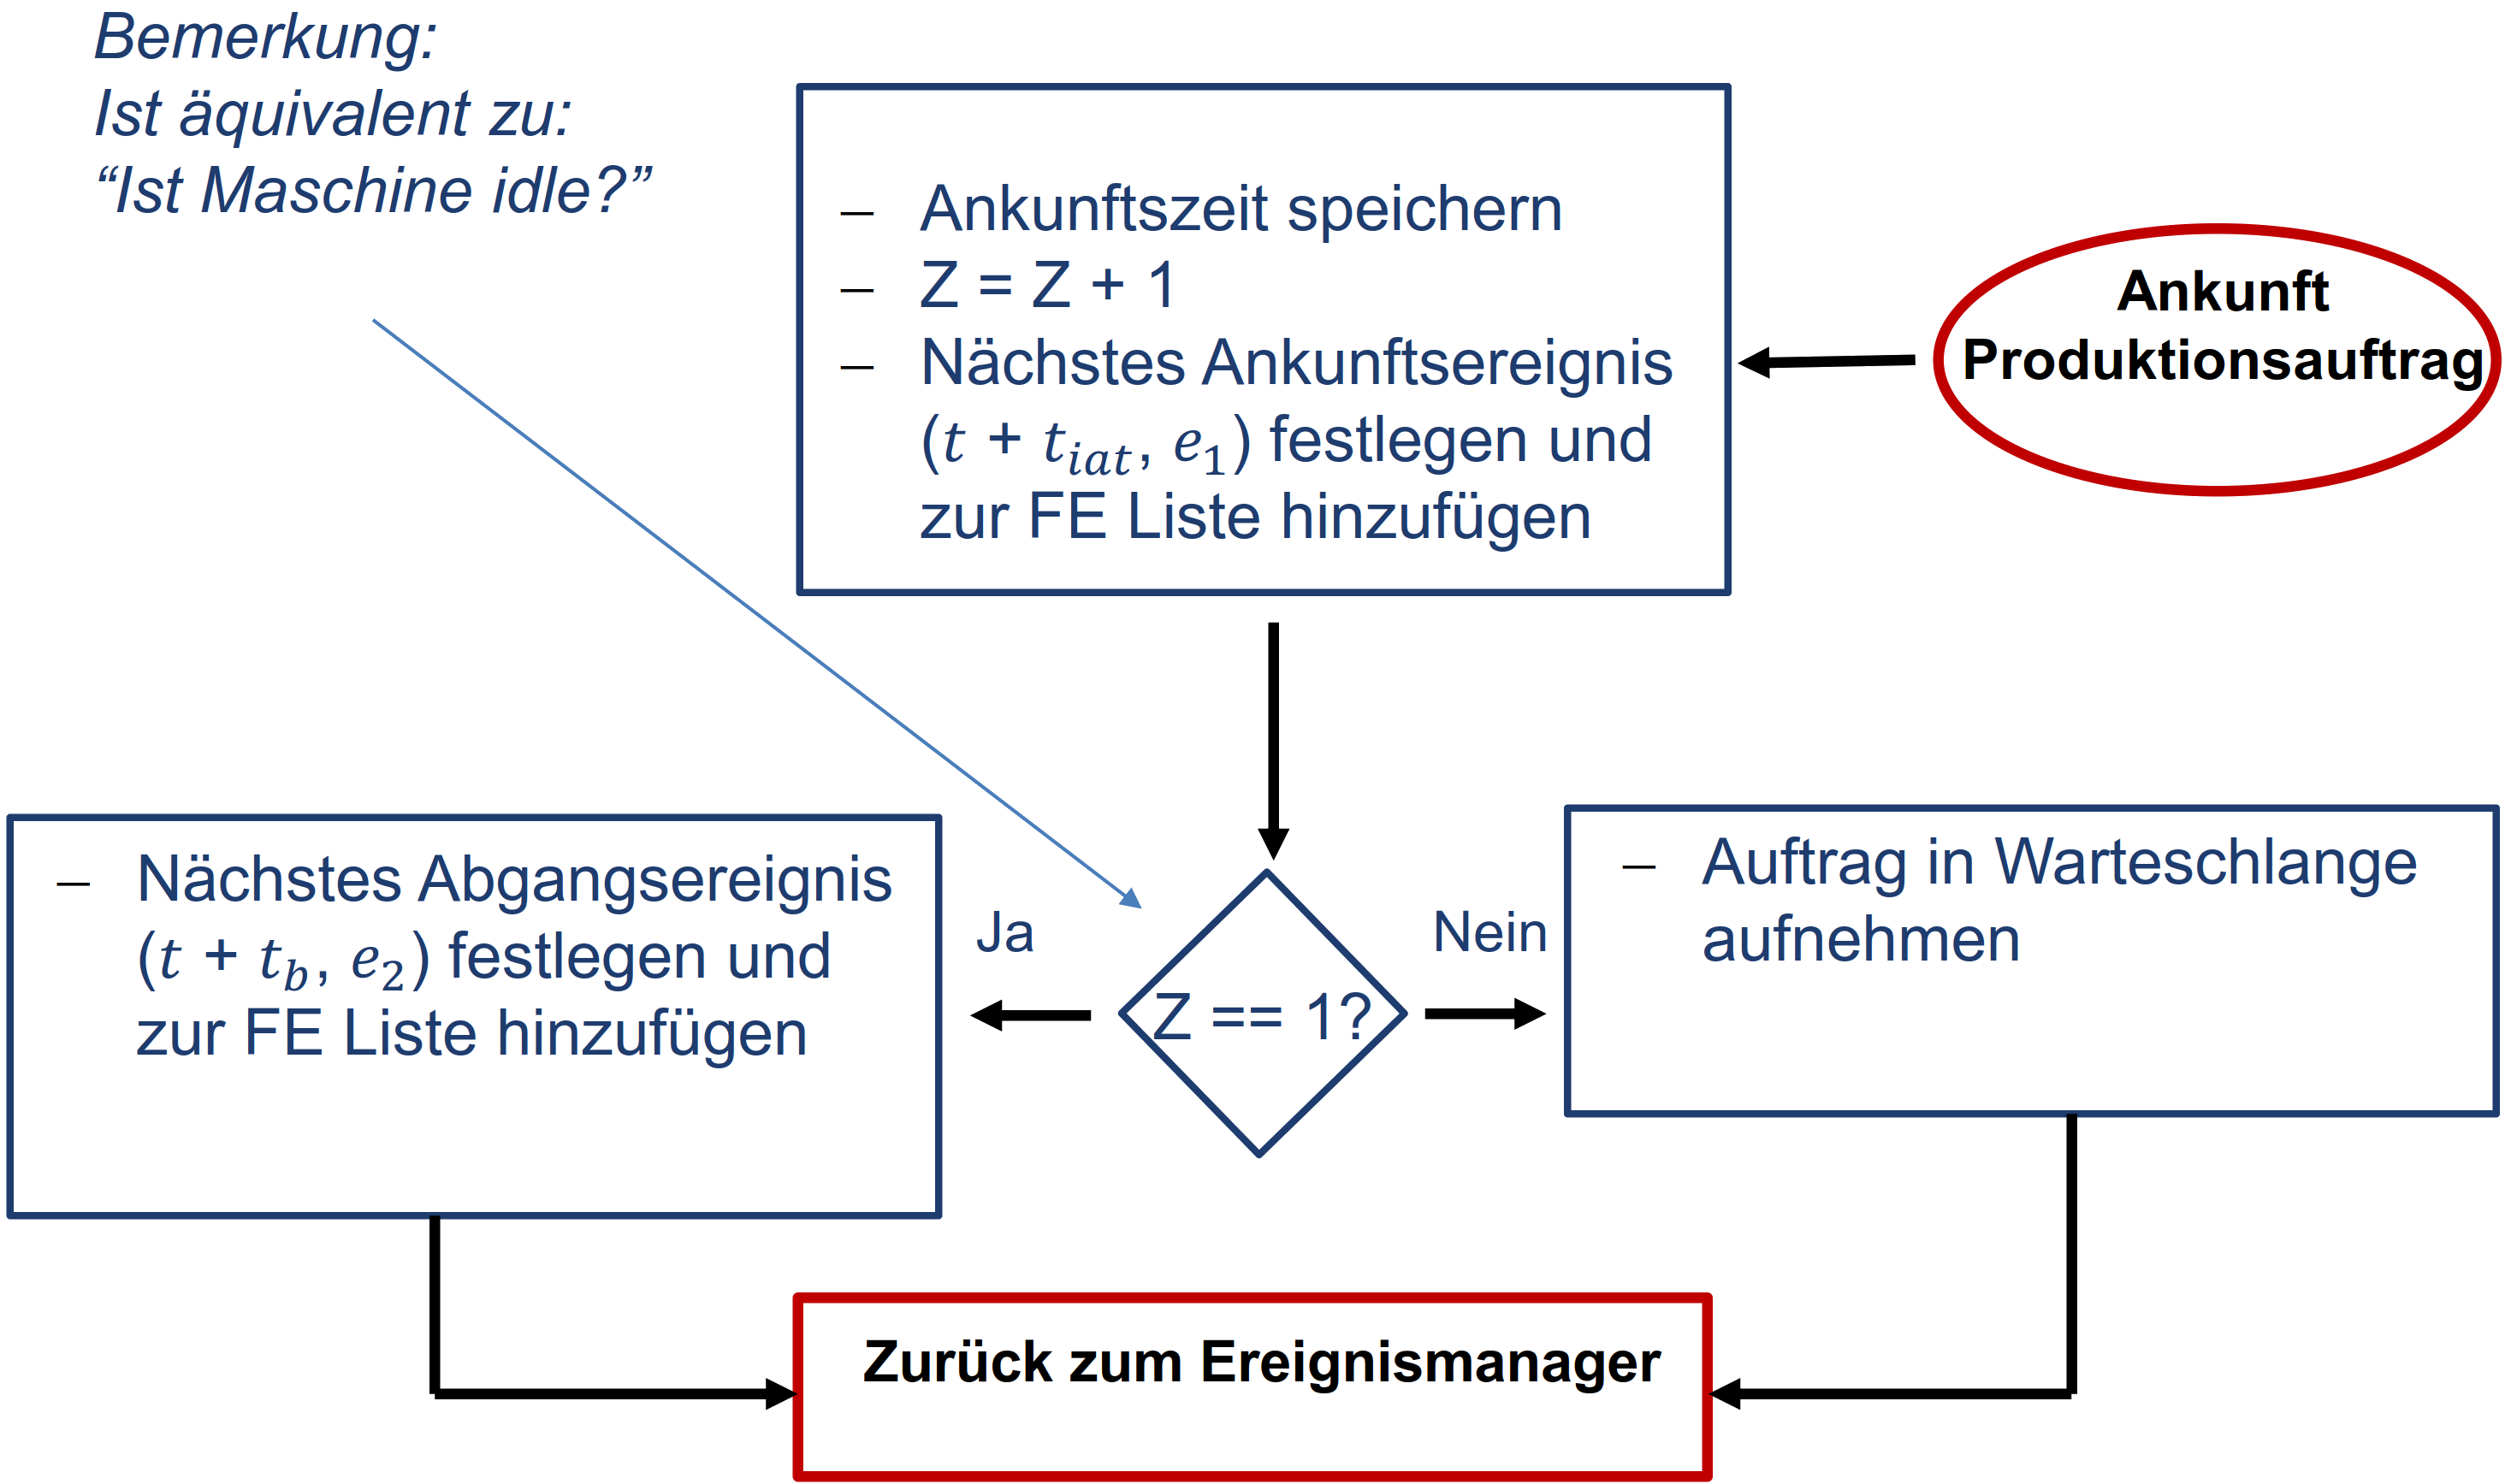
\includegraphics[width=0.5\textwidth]{pictures/ereignisdiagramm1}
		\textbf{Ereignisdiagramm $e_2$:} \\
		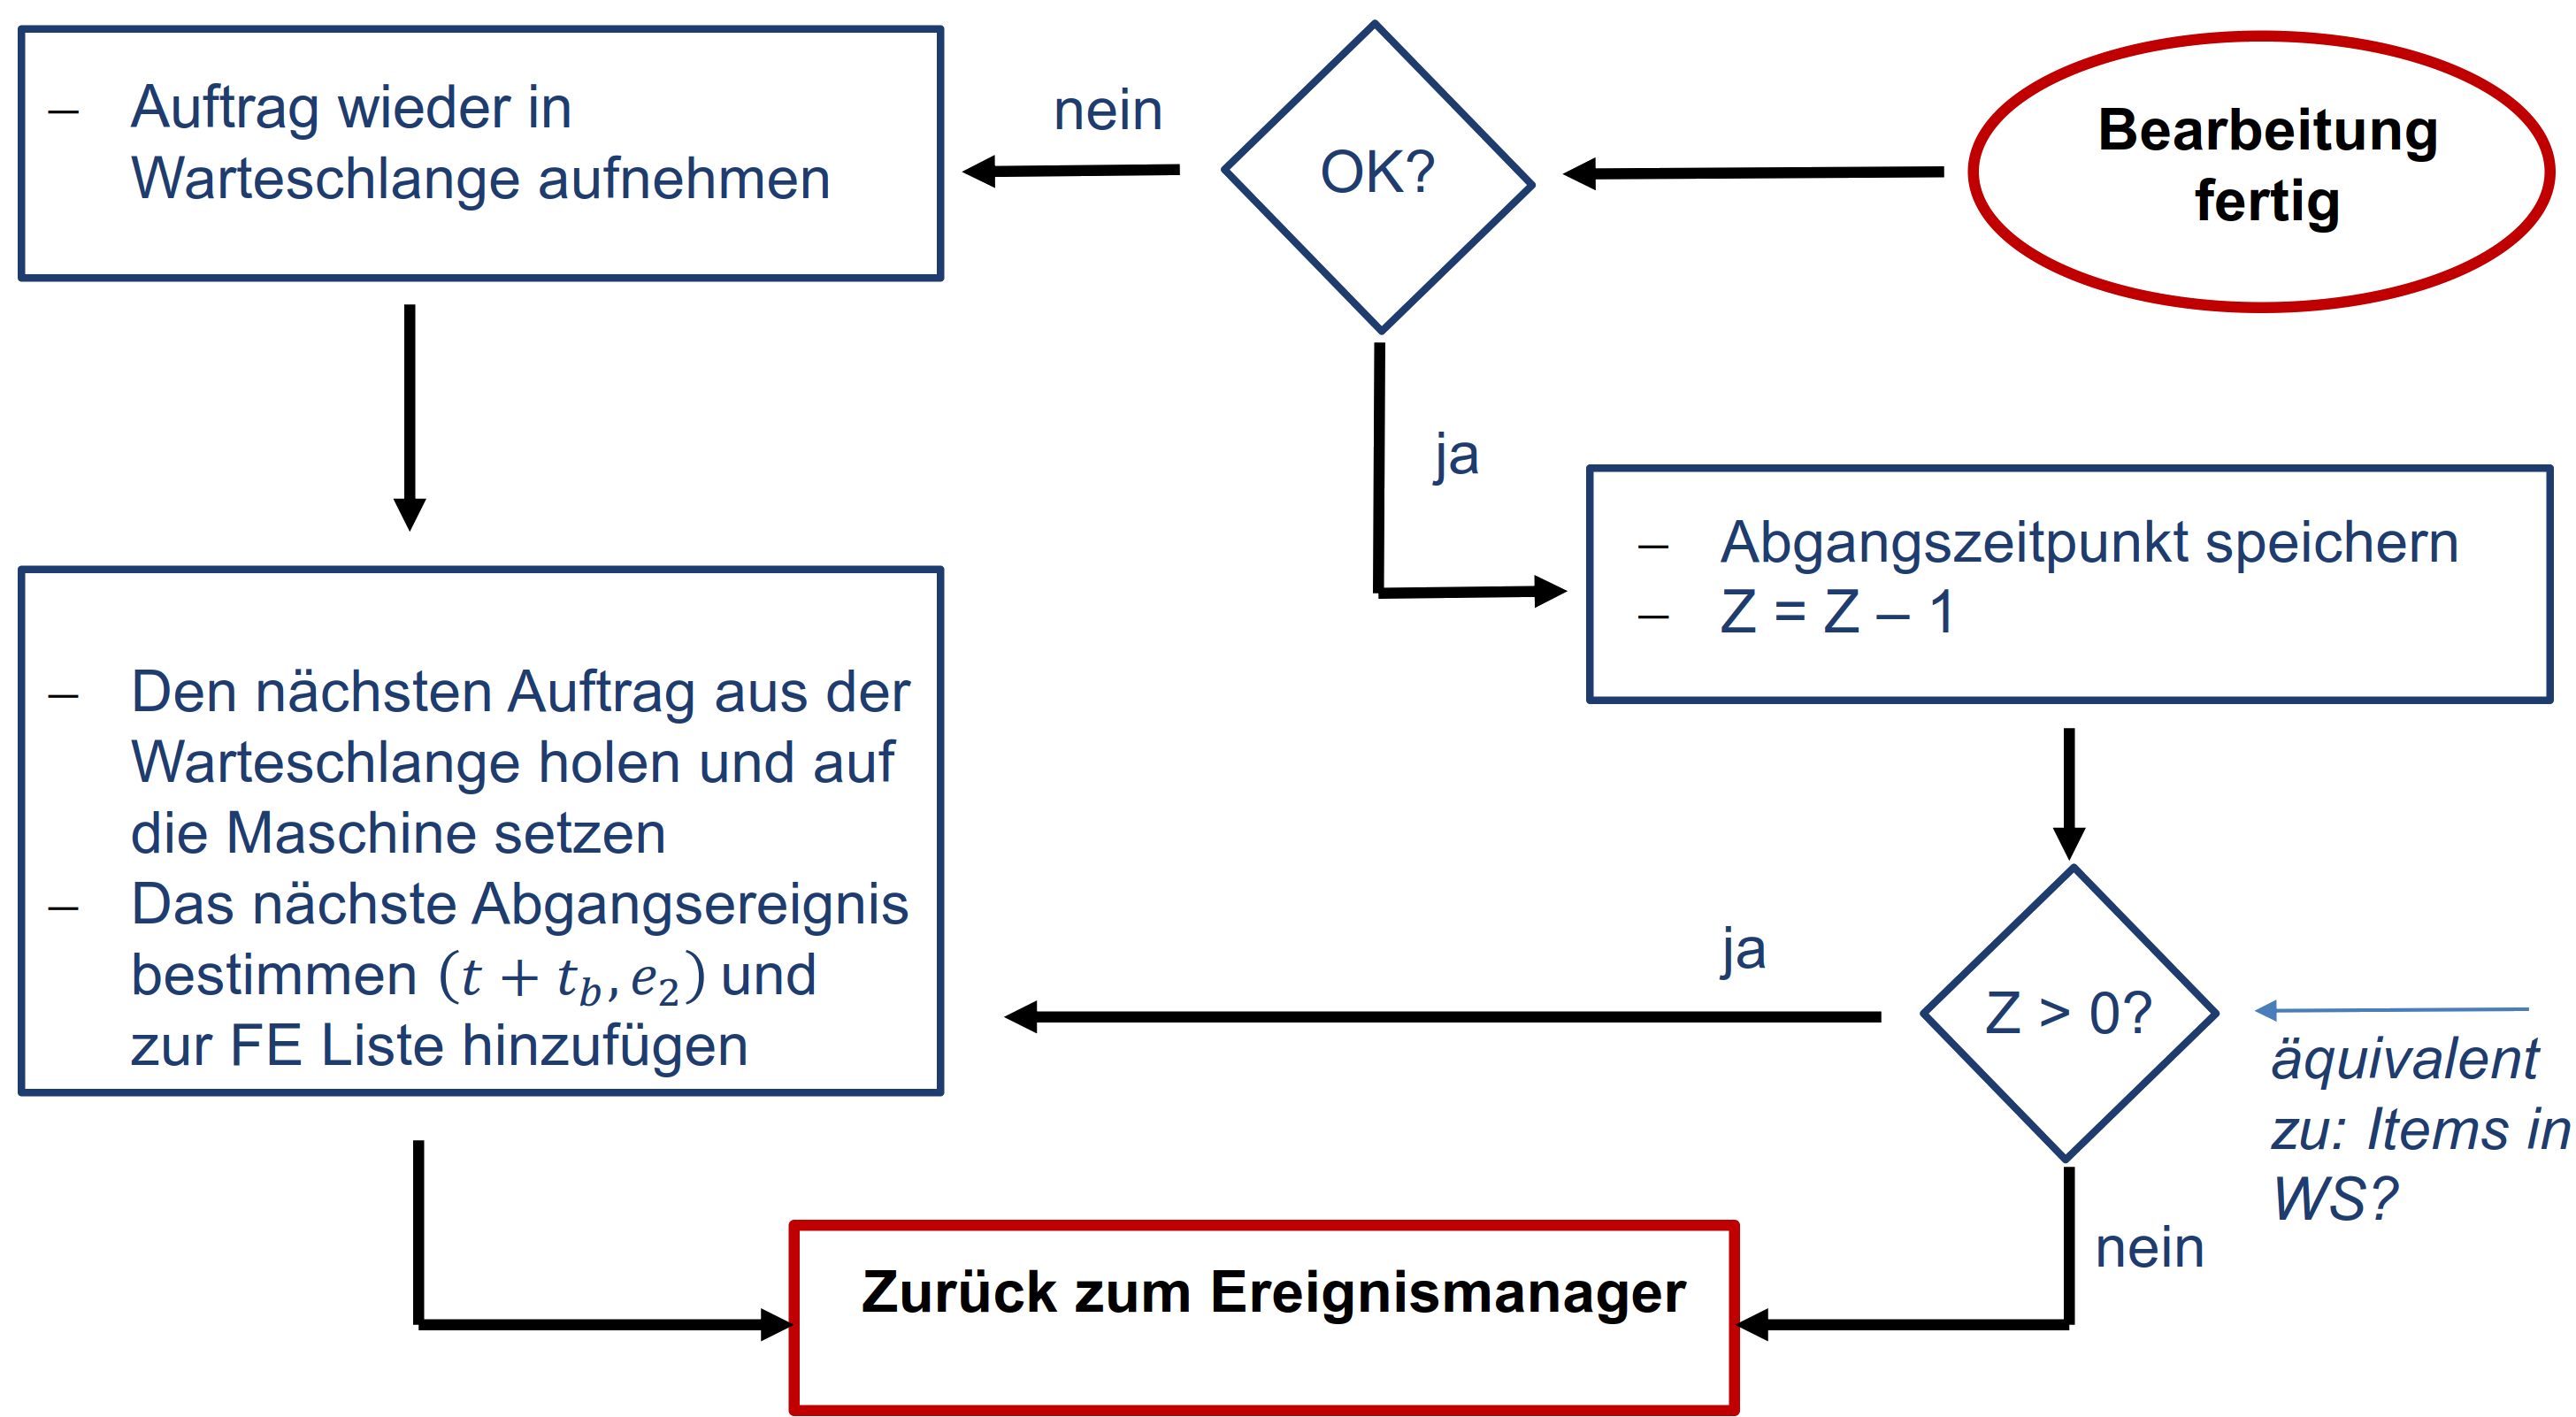
\includegraphics[width=0.5\textwidth]{pictures/ereignisdiagramm2}
	\end{multicols}
\end{example}

\subsubsection{Simulationskern / Ereignismanager}
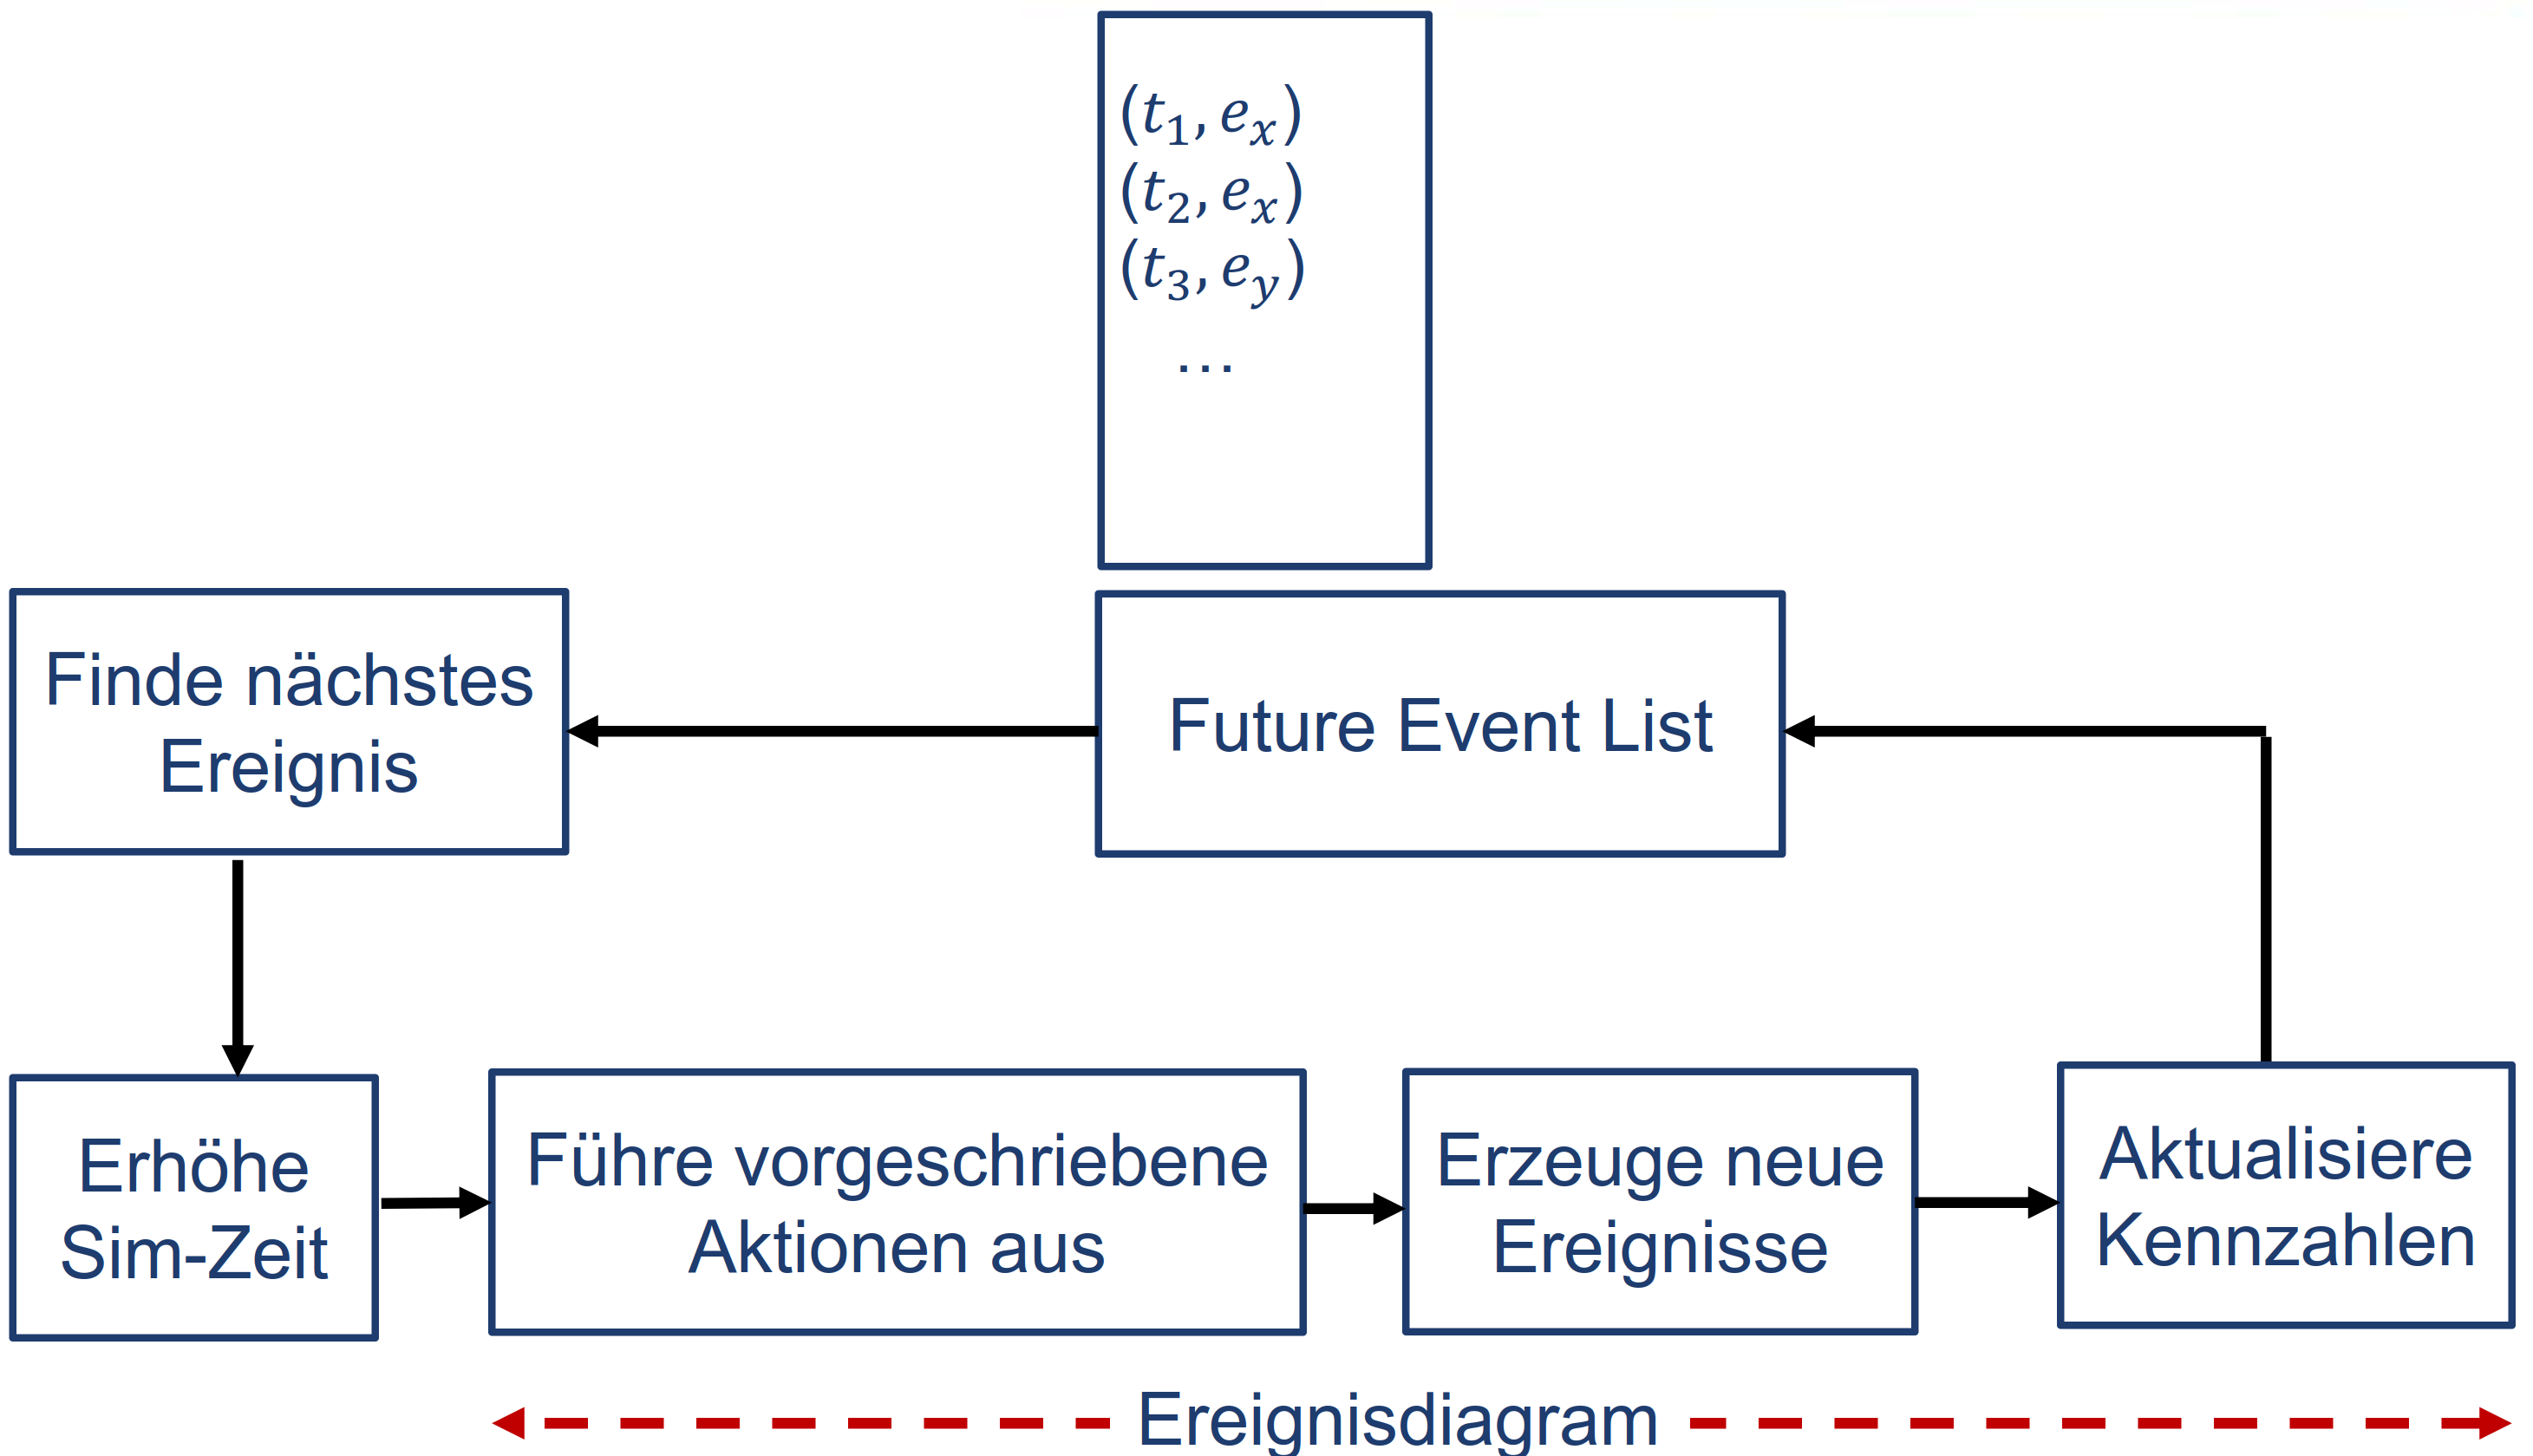
\includegraphics[width=0.5\textwidth]{pictures/ereignismanager}

\subsection{Wahrscheinlichkeitsverteilungen}	
\textbf{Vorteile:} 	
\begin{compactitem}
	\item Kompakte Formulierung (meistens 1 oder 2 Parameter)
	\item Leicht anzupassen (über die geringe Anzahl Parameter)
	\item Grosser Bereich an ausgewürfelten Zufallszahlen
\end{compactitem}	
\textbf{Nachteile:}
\begin{compactitem}
	\item Beschränkte Anzahl Parameter, um die Verteilung in die gewünschte Richtung anzupassen. Manchmal einfach nicht möglich, die komplexe Wirklichkeit in einer Verteilung mit 1 oder 2 Parametern abzubilden.
	\item Verteilung repräsentiert die Wirklichkeit oft nicht gut in Extremsituationen.
\end{compactitem}

\begin{multicols}{3}
	\subsubsection{Uniformverteilung} 
	$X \sim U[0, 200]$ \\
	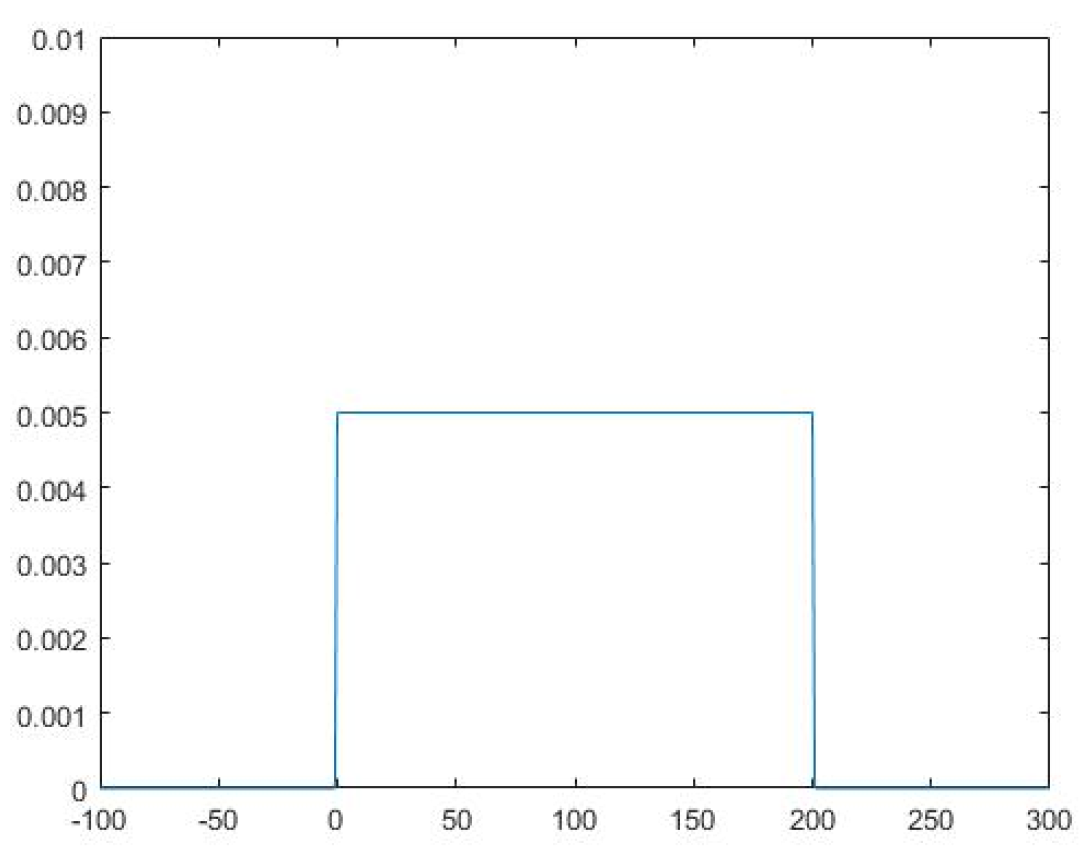
\includegraphics[width=0.25\textwidth]{pictures/uniformverteilung} 
	\subsubsection{Normalverteilung} 
	$X \sim N(100, 10'000)$ \\
	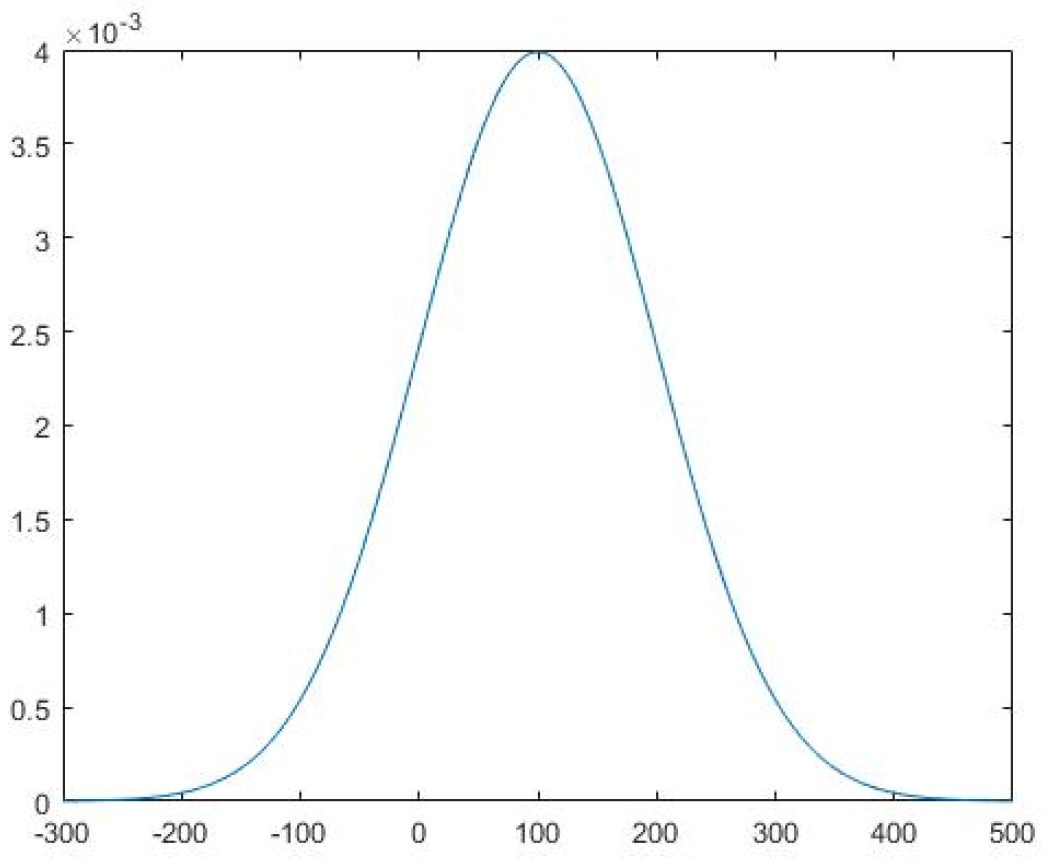
\includegraphics[width=0.25\textwidth]{pictures/normalverteilung} 
	\subsubsection{Poissonverteilung}
	$X \sim P(4)$ \\
	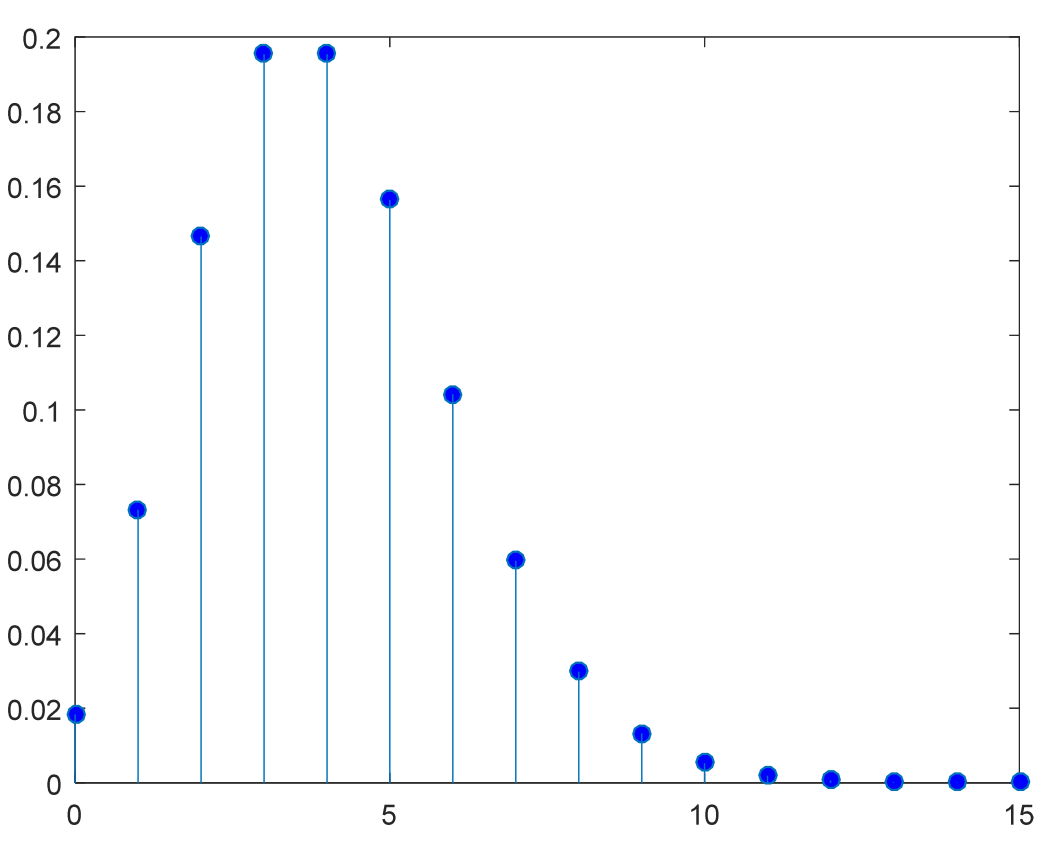
\includegraphics[width=0.25\textwidth]{pictures/poissonverteilung} 
\end{multicols}

\subsubsection{Empirische Verteilung}
\begin{multicols}{2}
	\begin{tabular}{|l|l|}
		\hline
		\textbf{Zufallszahl} & \textbf{Wahrscheinlichkeit} \\ \hline
		1 & 0.4 \\ \hline
		2 & 0.3 \\ \hline
		4 & 0.1 \\ \hline
		8 & 0.15 \\ \hline
		16 & 0.05 \\ \hline
	\end{tabular} \\
	\textbf{Vorteile:}
	\begin{compactitem}
		\item Basiert auf realen Daten
		\item Alle möglichen Formen sind möglich
	\end{compactitem}	
	\textbf{Nachteile:}
	\begin{compactitem}
		\item Es können keine Zufallszahlen erzeugt werden, die nicht schon in der Vergangenheit aufgetreten sind. Daher braucht man eine lange	Historie.
		\item Empirische Verteilungen kann man nicht kompakt auf Papier darstellen.
	\end{compactitem}
\end{multicols}

\subsubsection{Parameterschätzungen Gefahren}
\begin{multicols}{2}
	\begin{compactitem}
		\item Zu wenig Datenmaterial
		\item Nicht-repräsentative Vergangenheitsdaten
		\item Unberücksichtigte Ausreisser
		\item Unerkannte Zeitmuster (Sommer / Winter, Mo-Fr versus Sa-So)
		\item Falsche Interpretation des vorhandenen Datenmaterials
	\end{compactitem}
\end{multicols}

\subsection{Zufallszahlen}
\textbf{Grobe Definition:} Eine Bit-Reihenfolge ist willkürlich, wenn sie auf keine Weise ein Muster enthält. \\
\textbf{Zufallszahlengenerator:} Erzeugt Zufallszahlen zwischen 0 und 1 (und wandelt sie bei Bedarf in Zufallszahlen aus der gewünschten Wahrscheinlichkeitsverteilung um). \\ \\
\textbf{Anforderungen:}
\begin{multicols}{2}
	\begin{compactitem}
		\item Unabhängigkeit (auch die Elemente jeder Teilfolge)
		\item Gleichverteilung (empirische Verteilung weitgehend konstant)
		\item Besetzungsdichte (keine Lücken)
		\item Keine Periodizität
		\item Schneller und speichereffizienter Generator
		\item allenfalls Reproduzierbarkeit
	\end{compactitem}
\end{multicols}	
\textbf{Bemerkung:} Wirkliche Zufallszahlen sind nicht reproduzierbar. In den meisten Fällen will man die Zufallszahlen aber reproduzieren können. Wir sprechen in dem Fall von Pseudo – Zufallszahlen.
	
\subsubsection{Deterministische Reihenfolge}
\begin{compactitem}
	\item Jede Zufallszahl wird direkt aus ihrem unmittelbaren Vorgänger erzeugt.
	\item Die Erzeugung von Zufallszahlen startet mit einem initialen Wert. Dieser erste Wert des Zahlenflusses wird als Seed bezeichnet.
	\item Der Seedwert legt den gesamten Zahlenfluss eindeutig fest. D.h., wenn die Seedwerte identisch sind, sind die Zahlenflüsse, die sie auslösen, es auch.
\end{compactitem}

\subsubsection{Lineare Kongruenzmethode}
\textbf{Formel:} $X_{i+1}=(aX_i+c)\mod m$ mit $a$, $c$, $m$ und $X_0$ als Integer und $m > 0$, $a < m$, $c < m$ und $X_0 < m$ \\
somit gilt: $u_i = \frac{X_i}{m-1}\sim U(0, 1)$ \\
Die Qualität des Zufallszahlengenerators hängt stark von a, c und m ab. Die wichtigsten Parameter sind a und m; Meistens wählt man sehr hohe (Prim-)Zahlen. \\
\textbf{Problem:} In den allermeisten Fällen brauchen wir keine uniformverteile Zufallszahlen zwischen 0 und 1 sondern Zufallszahlen die aus einer anderen Verteilung stammen.

\subsubsection{Intervallmethode (Diskrete Zielverteilung)}
\begin{minipage}[h]{0.6\textwidth}
	\begin{tabular}{|l|l|l|l|}
		\hline
		\textbf{i} & \textbf{Zufallszahl}($r_i$) & \textbf{Wahrscheinlichkeit} & \textbf{Intervall} ($c_{i-1}$, $c_i$) \\ \hline
		1 & 1 & 0.4 & [0.00, 0.4) \\ \hline
		2 & 2 & 0.3 & [0.40, 0.7) \\ \hline
		3 & 4 & 0.15 & [0.70, 0.85) \\ \hline
		4 & 5 & 0.1 & [0.85, 0.95) \\ \hline
		5 & 18 & 0.05 & [0.95, 1.0) \\ \hline
	\end{tabular}
\end{minipage}
\begin{minipage}[h]{0.3\textwidth}
	\begin{lstlisting}[mathescape=true, tabsize=2]
x= U(0,1); // Standard Zufallszahl 
           // zwischen 0 und 1
for i = 1 : n
	if $c_{i-1}$ =< x < $c_i$
		returnValue = $r_i$;
		break;
	end
end
	\end{lstlisting}
\end{minipage}

\subsubsection{Inversionsmethode (Kontinuierliche Zielverteilung)}
\begin{compactenum}
	\item Generiere $x\sim U(0, 1)$
	\item Berechne $y = F_y^{-1}(x)$ 
\end{compactenum}
\begin{example}
	Uniformverteilung im Bereich [a, b] 
	\begin{multicols}{2}
		\begin{compactitem}
			\item Gegeben: $x\sim U(0, 1)$
			\item Gesucht: $y\sim U(a, b)$
			\item Transformation: $y = a+(b-a)x$
			\item Beachte: $F_y(y) = \left\{\begin{array}{ll}
												0 & y < 0 \\
												\frac{y-a}{b-a} & a \leq y < b \\
												1 & y \geq b \\
											\end{array}\right.$
		\end{compactitem}
		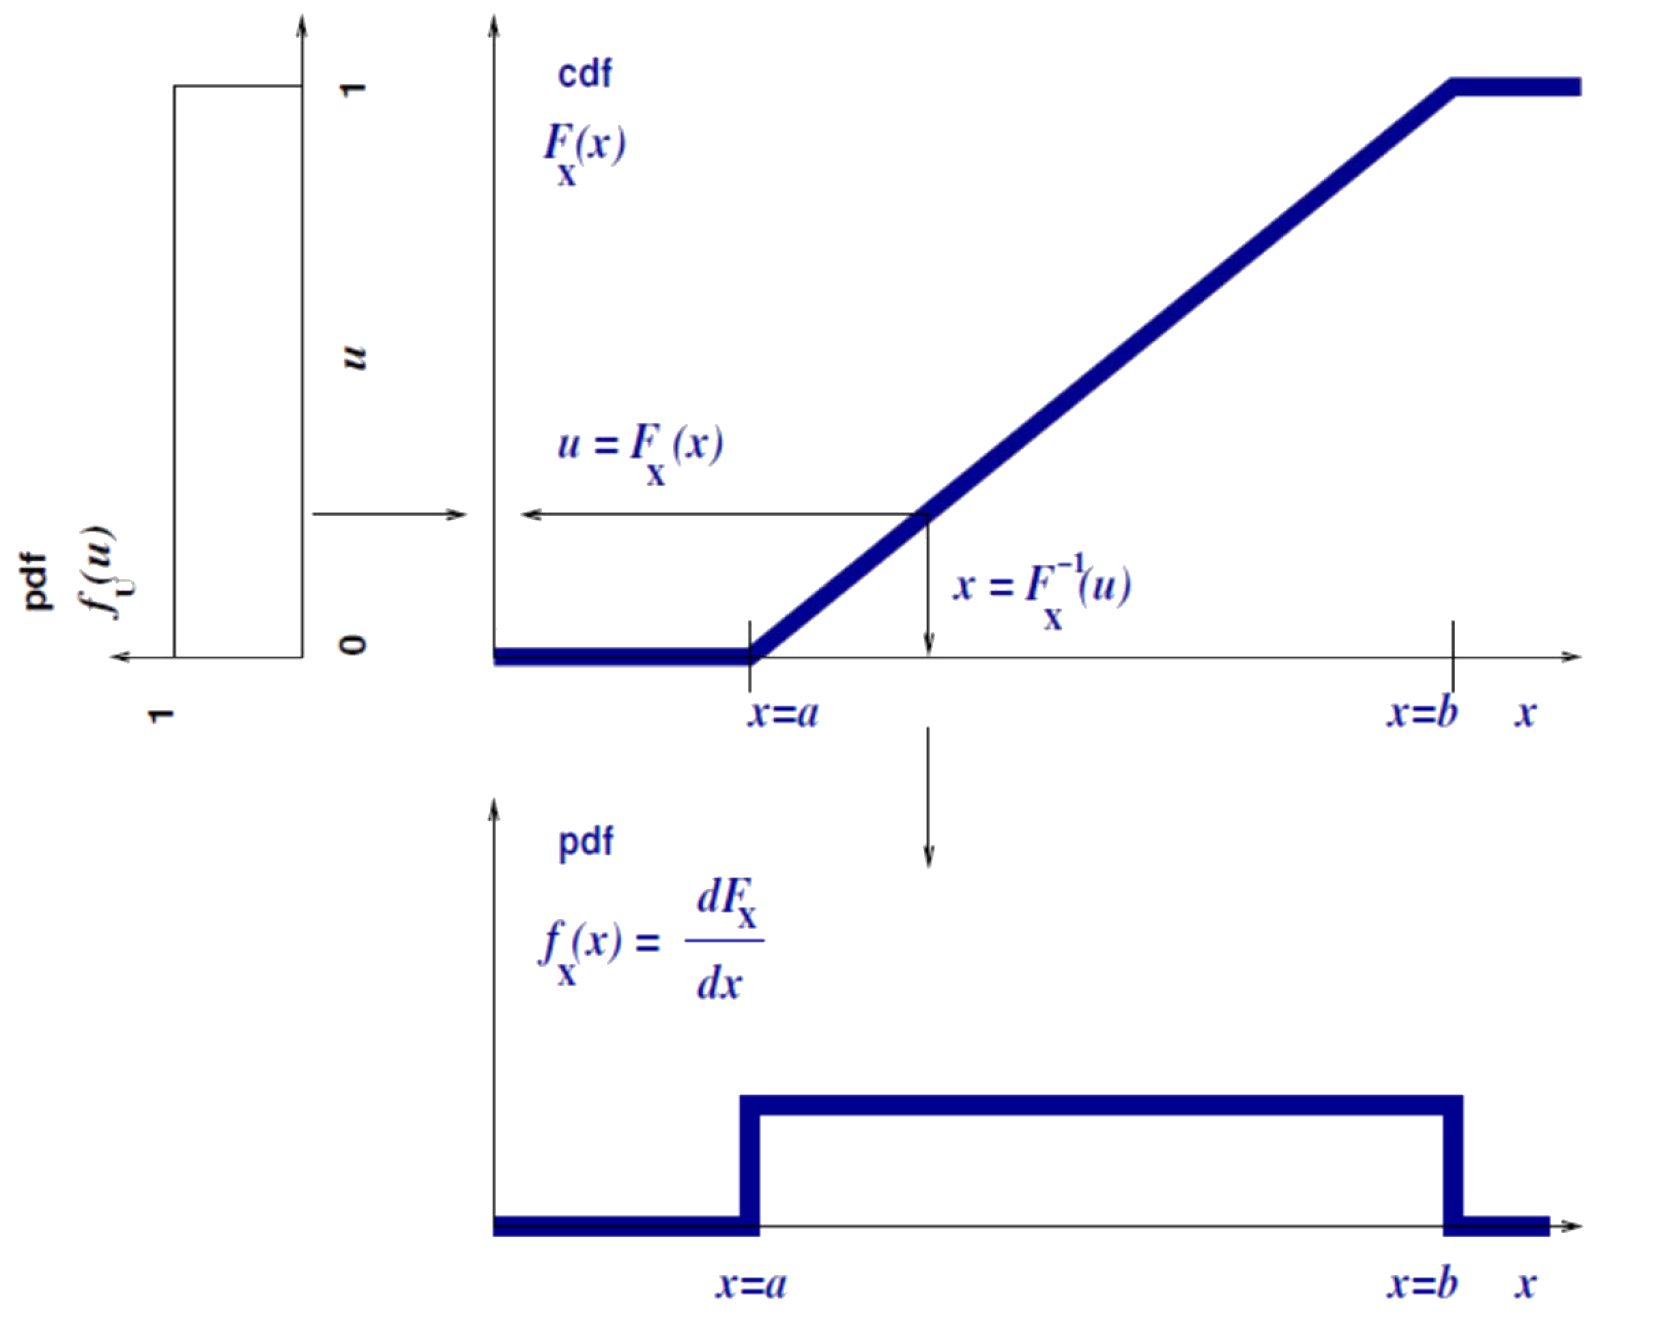
\includegraphics[width=0.33\textwidth]{pictures/inversionsmethode} 
	\end{multicols}
\end{example}

\begin{multicols}{2}
	\begin{example} 
		Exponentionalverteilung mit Parameter $\lambda$ \\
		\begin{compactitem}
			\item Gegeben: $x\sim U(0, 1)$
			\item Gesucht: $y\sim \exp (\lambda)$
			\item Beachte: $\begin{array}{l}
								F_y(y) = 1-e^{-\lambda y} \\
								x = 1-e^{-\lambda y} \\
								e^{-\lambda y} = 1-x\\
								y = -\frac{1}{\lambda}\ln (1-x)
							\end{array}$
		\end{compactitem}
	\end{example}
	\begin{example} 
		Empirische Verteilung \\
		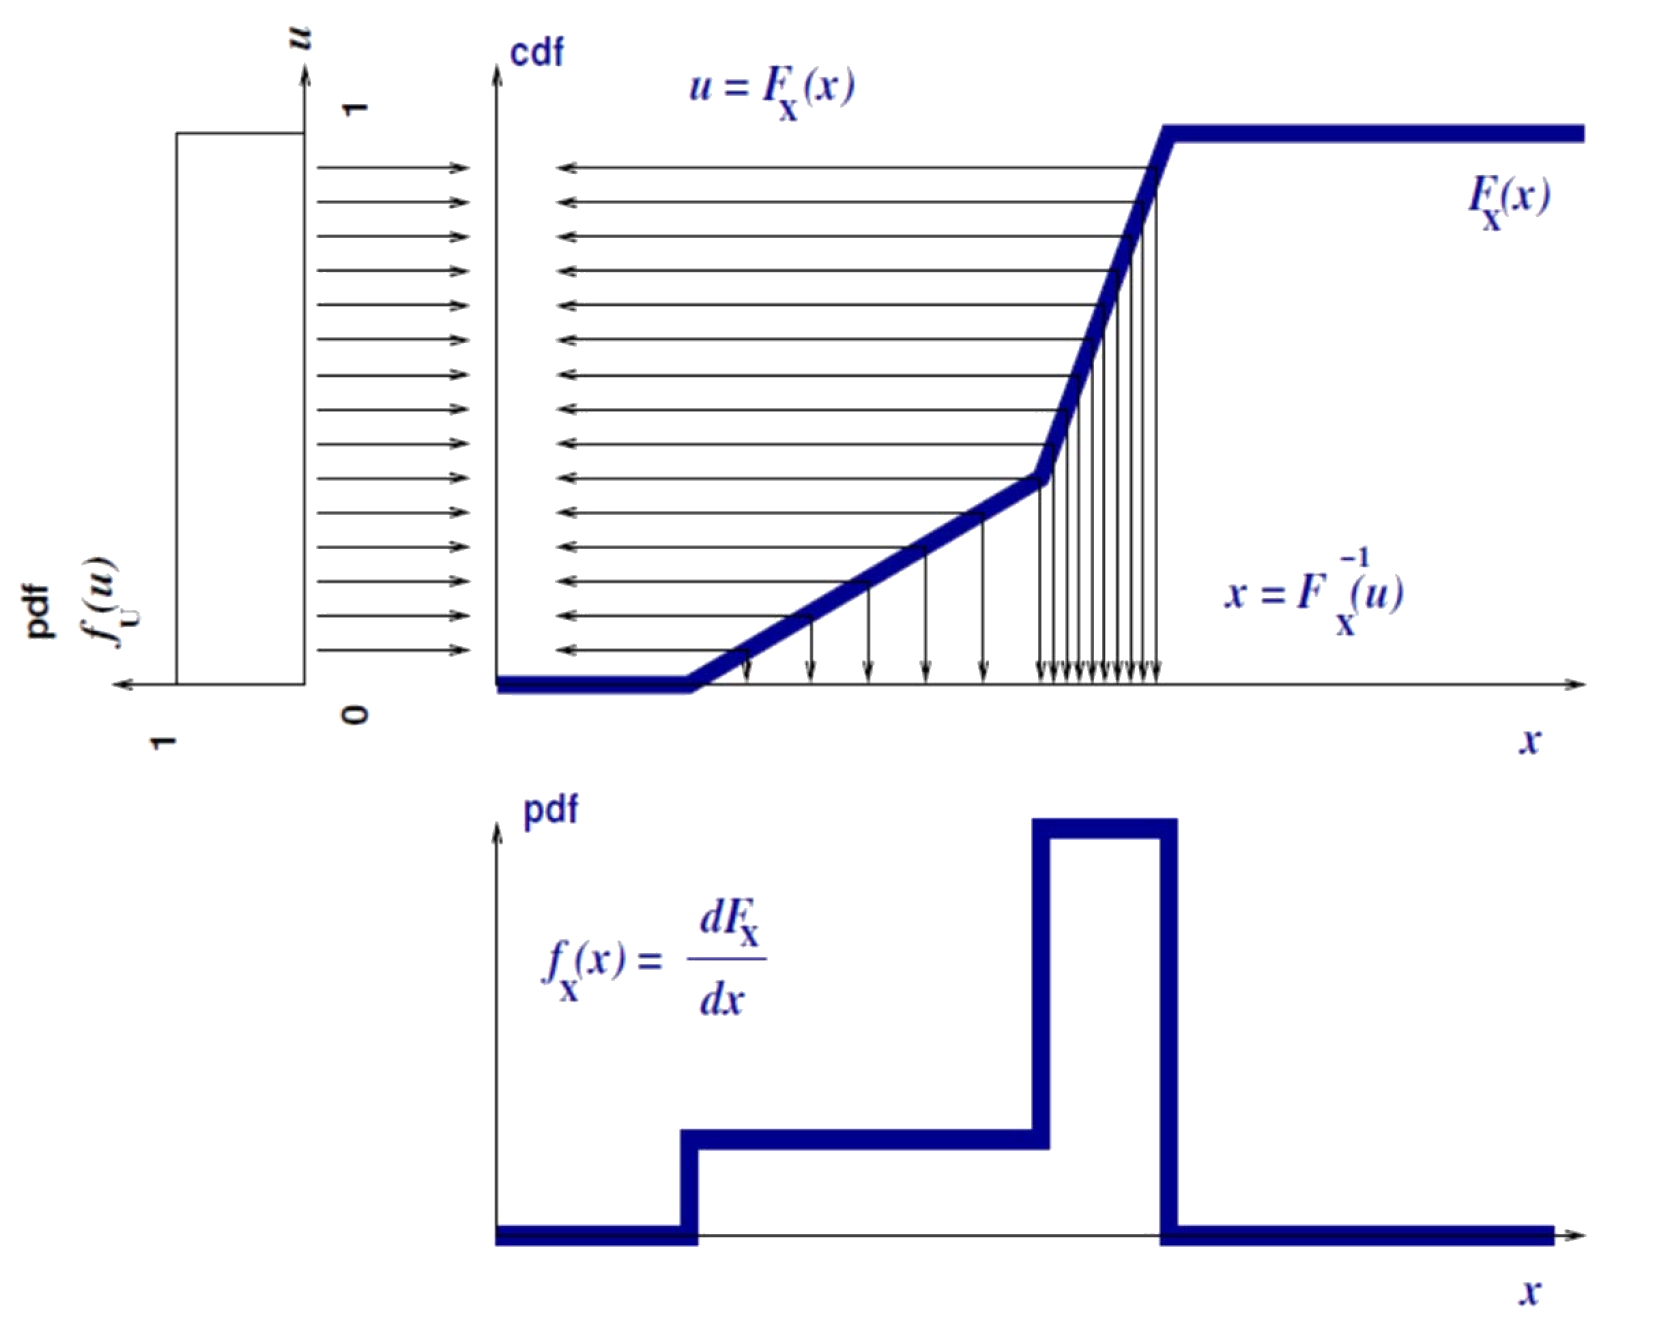
\includegraphics[width=1\textwidth]{pictures/inversionsmethode2} 
	\end{example}
\end{multicols}

\subsubsection{Wahl geeigneter Seedwerte}
\begin{compactitem}
	\item Der konkrete Seedwert spielt absolut keine Rolle (1, 2 oder 25343).
	\item Wichtig ist, ob Seedwerte identisch oder nicht-identisch sein sollten.
	\item Innerhalb eines Simulationslaufs: UNTERSCHIEDLICH
	\item Wenn wir 2 verschiedene Szenarien vergleichen wollen, wählen wir allerdings mit Vorteil Seed-Sätze, die identisch sind, um somit den \aszeichen{Zufallseinfluss} so weit wie möglich zu minimieren.
\end{compactitem}

\subsection{Ergebnisanalyse}
Simulationsergebnisse (z.B. durchschnittliche Wartezeiten in einer Arztpraxis) sind abhängig von Zufallszahlen (z.B. Behandlungsdauer, Zwischenankunftszeiten, usw.). Jedes Simulationsexperiment erzeugt neue Ergebnisse (solange Seed-Werte nicht fixiert sind). Simulationsergebnisse sind somit selbst auch Zufallszahlen!

\subsubsection{Konfidenzintervall}
Ein Konfidenzintervall (auch Vertrauensbereich oder Vertrauensintervall) ist ein Intervall aus der Statistik, das die Präzision der Lageschätzung eines Parameters (zum Beispiel eines Mittelwertes) angibt. Das Konfidenzintervall ist der Bereich, der bei unendlicher Wiederholung eines Zufallsexperiments mit einer gewissen Häufigkeit (dem Konfidenzniveau) die wahre Lage des Parameters einschliesst.
\begin{example}
	Die Anzahl Wanderer zwischen 9 und 10 Uhr morgens an der Talstation der Säntisbahn an einem sonnigen Tag in den Sommerferien bewegt sich mit einer Wahrscheinlichkeit von 95\% zwischen 50 und 200.\\
	Mathematisch: $P(X \in [50,200]) =  0.95$
\end{example}

\subsubsection{Batch-Mittelwert-Methode}
\begin{compactenum}
	\item Nach Einschwingverhalten, Gesamtzeit (resp. Gesamtmenge von Beobachtungen) in $n$ gleiche Batches teilen
	\item Mittelwert pro Batch berechnen
	\item Einzelmittelwerte mitteln (sofern Batches unabhängig voneinander sind, ist bei genügend langen Batches der Fall)
	\item Aus Streuung der Einzelmittelwerte Vertrauensintervall für Mittelwertschätzer bestimmen
\end{compactenum}
\begin{minipage}[h]{0.8\textwidth}
	\textbf{Mittelwert pro Batch:} $\hat{\theta}_i$\\
	\textbf{Einzelmittelwert:} $\hat{\theta}_n=\frac{1}{n}\sum_{i=1}^{n}\hat{\theta}_i$\\
	\textbf{Streuung:} $S_n^2=\frac{1}{n-1}\sum_{i=1}^{n}(\hat{\theta}_i-\hat{\theta}_n)^2$ \\
	\textbf{Konfidenzintervall:} $\hat{\theta}_n-z_{\frac{\alpha}{2}}\sqrt{\frac{\sigma^2}{n}} < \theta < \hat{\theta}_n+z_{\frac{\alpha}{2}}\sqrt{\frac{\sigma^2}{n}}$ mit $n$ = Anzahl Batches \\
	\textbf{Interpretation für n $>$ 29:} $P(\theta \in [\hat{\theta}_n-z_{\frac{\alpha}{2}}\sqrt{\frac{\sigma^2}{n}}, \hat{\theta}_n+z_{\frac{\alpha}{2}}\sqrt{\frac{\sigma^2}{n}}])=1-\alpha$
\end{minipage}
\begin{minipage}[h]{0.2\textwidth}
	\begin{tabular}{|l|l|}
		\hline
		$\alpha$ & $z_{\frac{\alpha}{2}}$ \\ \hline
		0.1 & 1.645 \\ \hline
		0.05 & 1.96 \\ \hline
		0.01 & 2.576 \\ \hline
	\end{tabular}
\end{minipage}	